%\setcounter{chapter}{2}


%    https://tex.stackexchange.com/questions/40725/how-to-change-the-font-size-during-the-new-defined-environment
%    http://www.sascha-frank.com/latex-font-size.html
\begin{normalsize}
%\begin{small}
%\begin{footnotesize}



\chapter{LHC and the CMS experiment}
\label{ch:cms}
CERN accelerator complex is a sequence of machines that produces and accelerates "bunches" of $10^{11}$ protons to nearly the speed of light. In the Large Hadron Collider (LHC) the bunches collide at specific interaction points (IP), where the four main experiments are located: ALICE, ATLAS, CMS, and LHCb. We will start this section with the discussion of the LHC machine and then describe the CMS detector. 

\section{The Large Hadron Collider}\label{sec:cms_intro}

%%%%%%%%%%%%%%%%%%%%%%%%%%%%%%%%%%%%%%%%%%%%%%%%%


\subsection{The history of the LHC}

The story of the LHC begins in 1977, when the CERN director general Sir John Adams suggested that the tunnel of the Large Electron-Positron Collider (LEP) can be reused to accommodate the future hadron collider of more than 3 TeV energies \ref{Sadenius}. At the 1984 ECFA-CERN workshop on a "Large Hadron Collider in the LEP Tunnel" \ref{LHC1984}, the physics goals of the LHC were stated: confirmation of the BEH mechanism, search for the Higgs Boson, and exploration of the origin of masses of W and Z bosons. The parameters of the proposed LHC were very ambitious: the centre-of-mass (COM) collision energy of 10 to 20 TeV, and a target instantaneous luminosity of 10$^{33-34}\frac{1}{cm^{2}s}$. 

Large Hadron Collider (LHC) is the most powerful particle accelerator that has ever been built. It is located at the border of France and Switzerland at a depth from 50 to 175 m underground. LHC ring is 26.7 km in circumference and it is the final stage in a sequence of accelerators. 


\begin{figure}[H]
  \centering
%  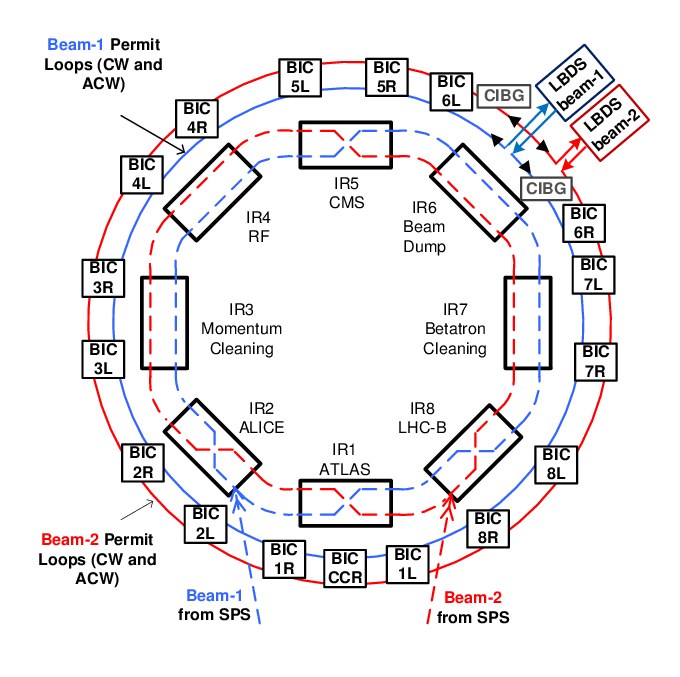
\includegraphics[width=0.75\textwidth]{LHC-beam-permit-loops}\\
  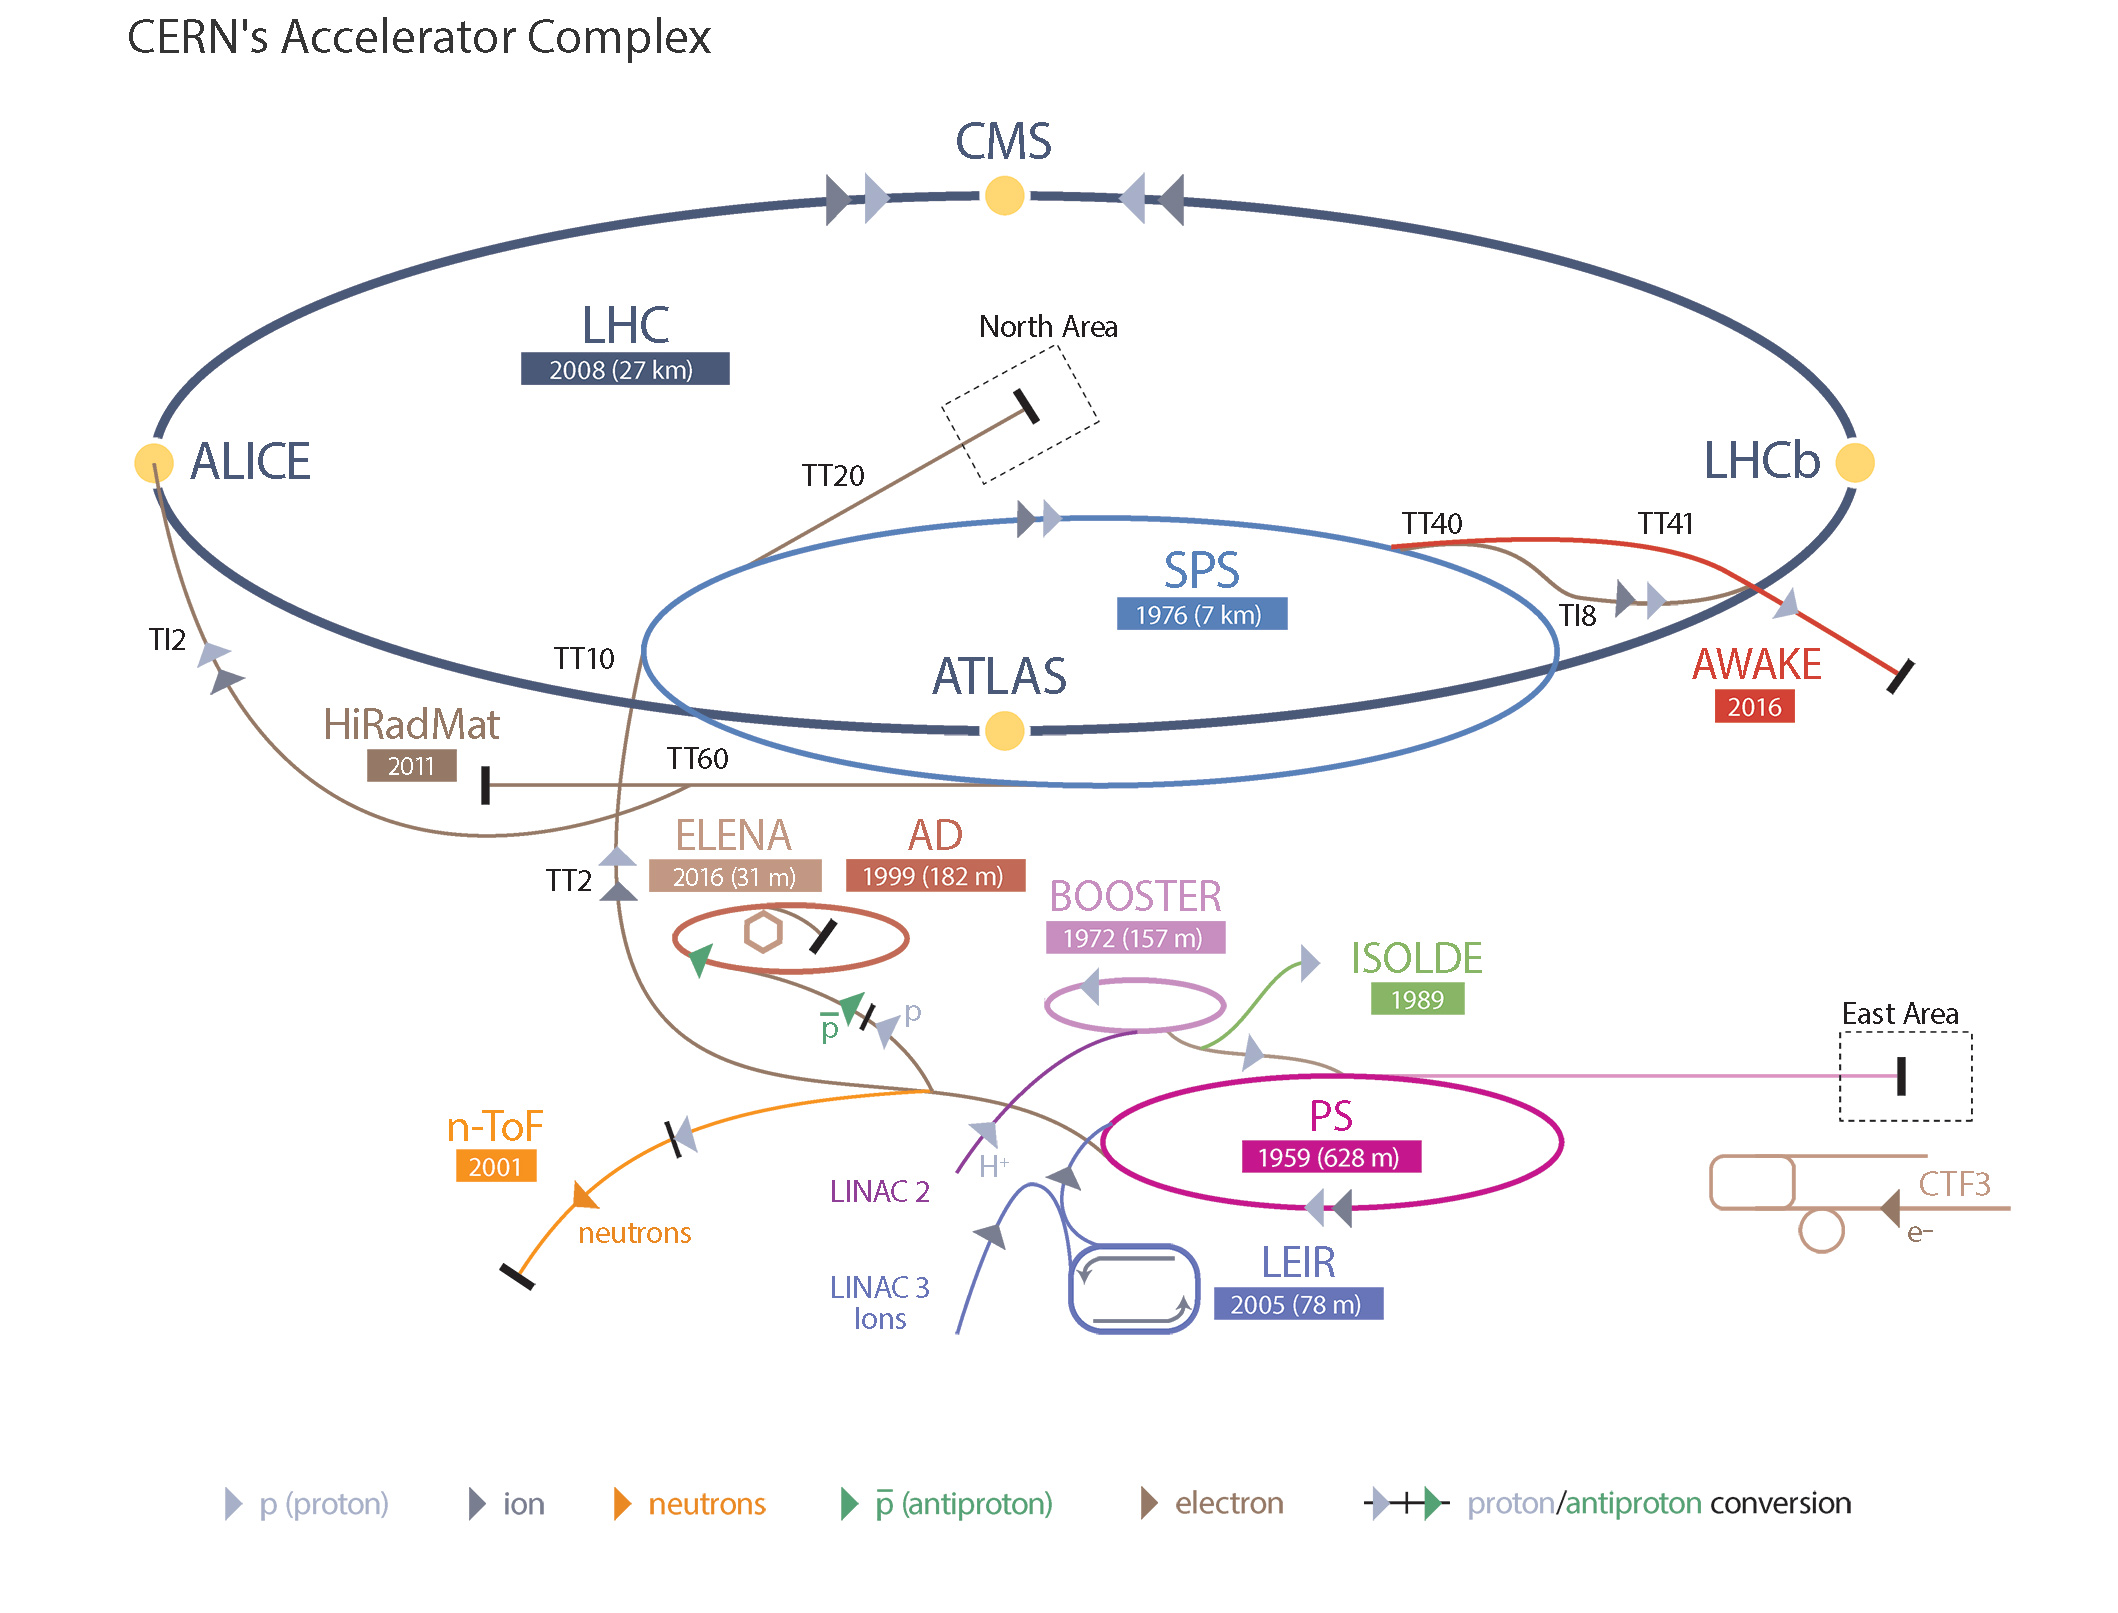
\includegraphics[width=0.75\textwidth]{LHC_default.jpg}
  \caption {Schematic layout of the LHC.}
  \label{lhcmap}
\end{figure}

%%%%%%%%%%%%%%%%%%%%%%%%%%%%%%%%%%%%%%%%%%%%%%%%%


\subsection{The layout of the LHC}

It is a complex process to start proton-proton collision in the LHC at 13 TeV and, therefore, the process consists of several stages (see Fig. \ref{lhcmap}). Everything begins with the bottle of hydrogen. The hydrogen atoms from the bottle are fed into the source chamber of the Linear Accelerator (Linac). In the chamber the hydrogen is heated up to the plasma state until electrons are stripped off of the hydrogen atoms. Then electrons are removed and remaining protons are directed to the first acceleration stage which increases the energy of protons to 50 MeV. After Linac, the beam of protons is injected into the Proton Synchrotron Booster (PSB). PSB contains four rings each accelerating a bunch of protons (a moving collection of protons of a narrow length) to 1.4 GeV. The third stage is the Proton Synchrotron (PS), which splits the incoming beam into 72 bunches separated by 7.5 m. The energy of the protons is increased to 25 GeV. After that, the protons are sent to the Super Proton Synchrotron (SPS), where they are accelerated to 450 GeV. SPS then fills the LHC ring with two beams each consisting of 2808 bunches of protons with nearly $10^{11}$ protons in total. It takes SPS about $O(10)$ minutes to fill each LHC ring with bunches. In the LHC two beams are circulating in opposite directions in two separate beam pipes. During standard data taking beams circulate for $O(10)$ hours.  

%%%%%%%%%%%%%%%%%%%%%%%%%%%%%%%%%%%%%%%%%%%%%%%%%

\subsection{LHC operations}

The first LHC budget plan was finalised in 1996 and the final cost was approved just a few years later. The first proton beam entered the LHC ring in 2008. However, an incident intervened the LHC plans. It was caused by the mechanical damage of the tunnel equipment due to the release of the helium. Thus, the real data taking period (called LHC Run-1) had started only in 2010 and lasted for two years with 7-8 TeV COM energies. The recorded dataset contained enough Higgs bosons to claim a discovery of this rarely produced particle. After this achievement, the LHC was closed for the first long shutdown (LS1) that happened in 2012. During this time necessary upgrades of the main detectors and the LHC were performed. This was an unavoidable and essential step to prepare the LHC for more challenging environment of COM energies increased to 13 TeV. 


If we denote the area of 10$^{-28}$ $m^2$ as barn (b), then in terms of these new units the LHC can theoretically produce $80-120/fb$ of data a year. In practice numbers were lower, because LHC operated at the revolution frequency below the nominal, used fewer proton bunches in the beam, etc.  All this resulted in lower than expected instantaneous luminosity, which is a very important term in collider physics and will be explained in the next section.

The LHC Run-2 has started in 2015 and the CMS collected 4.2 $fb^{-1}$ of data that year. Over the course of the 2016 data taking, an integrated luminosity of 35.9 $fb^{-1}$ was recorded. This luminosity is the amount of data that has been collected by the CMS detector and later approved by the CMS physics coordination for the use in the physics analyses. The data set of proton-proton collisions collected in 2016 at 13 TeV COM energy is used in this thesis to analyse double Higgs boson decays. Together with the 2017 and 2018 data taking, almost 150 $fb^{-1}$ have been delivered and recorded by the CMS detector during the whole Run-2 period of four years. 

At the moment of writing this thesis, the LHC has entered the LS2. The next data taking will resume in 2020 and proton-proton collisions will continue for three years with the expected delivered integrated luminosity equal to nearly 300 $fb^{-1}$. This will conclude the LHC Phase-1 programme. 

The new upgraded LHC, the High-Luminosity LHC (LHC) or the Phase-2, will start operations in 2026 and run until 2035. The COM energy will be increased to 14 TeV and one expects to record an unprecedented dataset of 3000 $fb^{-1}$. 

\subsection{Luminocity}

%%%%%%%%%%%%%%%%%%%%%%%%%%%%%%%%%%%%%%%%%%%%%%%%%

The instantaneous luminosity is the coefficient which relates the cross section $\sigma$ of the process to the number of events $N_{events}$ produced during the interaction: $N_{events} = \mathcal{L}  \sigma$. Luminosity is the parameter controlled by the machine and can be written as:

$ \mathcal{L} =\frac{N^2 n_b f_{rev}}{4\pi \sigma_x \sigma_y}$

\noindent where $N_b$ is the number of particle in the colliding bunch, $n_b$ is the number of colliding bunches in the beam, $f_{rev}$ is the revolution frequency of the beam, $\sigma_x$ and $\sigma_y$ are the standard deviations of the beam density profile (BDP) in the transverse plane, where it is assumed that the BDP of both beams can be described by a Gaussian distribution.


To maximise the amount of collected data, the luminosity parameter should be as high as possible. It is worth noting that the luminosity is not constant and decays with time due to the degradation of the initial circulating beams. Theoretical decay time (the time to reach $1/e$ level) is approximately 29 h. In practice, taking into account the decrease of protons in the bunch due to collisions, contributions from the intrabeam scattering, scattering on the residual gas, etc., the real luminosity lifetime is about 15 h. 

A useful variation of the luminosity parameter is a total integrated luminosity. This is the number normally quoted for the dataset collected over the period T:

$L = \int_{0}^{T} \mathcal{L}  dt$.

In collider physics the "beam dump" is a process of burning off exhausted low luminosity beams by intentionally directing them towards the target made of concrete and steel. The time from the start of the collisions to the beam dump is usually called the "run".

We can calculate the amount of data delivered by the LHC during a single run period $O(10)$ h. Performing the integration, we obtain: 

 $L = \mathcal{L}_0 \tau_\mathcal{L}  \left[  1- e^{\frac{-\tau_{run}}{\tau_\mathcal{L} }}  \right]$, 

\noindent where $\mathcal{L}_0$ is the initial peak instantaneous luminosity at the start of the run, $\tau_{run}$ is the total duration of a run, and $\tau_\mathcal{L}$ is the luminosity lifetime. The optimum run time is 12 hours. During the runs, the LHC centre needs to dump the old beams, fill the rings with the new beams, and increase ("ramp") the energy of new beams to 13 TeV. After that a new run can be started. This restarting process normally takes two to six hours.

%%%%%%%%%%%%%%%%%%%%%%%%%%%%%%%%%%%%%%%%%%%%%%%%%


\subsection{LHC infrastructure}

The equipment of the LHC tunnel serves several purposes with the main objective to keep the colliding beams on the circular orbit. This requires a complex synchronised work of bending dipole magnets, cooling systems, accelerating radio frequency cavities, and vacuum insulation systems.

%%%%%%%%%%%%%%%%%%%%%%%%%%%%%%%%%%%%%%%%%%%%%%%%%

\subsubsection{Magnets}\label{sec:magnets}

Most of the LHC circumference is used by 1232 superconducting magnets placed evenly around the tunnel to approximate the circular orbit. These are dipole magnets (see Fig. \ref{dipoles_coils}) that bend the beam and keep it on the circular orbit, that is why they are commonly called "Main Bends" (MB). The proven technology existed since Tevatron and relied on NbTi superconductors. This technology also satisfied the LHC cost and performance requirements, thus, it was decided to reuse the same choice of the alloy for the LHC superconducting dipole magnets that steer the proton beams. 

The dipoles need to produce the magnetic field of 8.3T. % and it requires a current of about 11kA. 
Each dipole is 16.5 $m$ (with ancillaries) long and 570 $mm$ in diameter and is placed inside of the dipole cryostat which is called the "Helium bath". 

This cryostat is a long cylindrical tube 914 $mm$ in diameter made of low-carbon steel, where the dipole mass is cooled down to 1.9 $K$. Even though the inner structure of such cryostat is very complex and includes two beam pipes, two sets of coils for two beam pipes, vacuum pipes etc., one normally calls this compound object simply a dipole magnet. The name "dipole" is reserved for MBs since for each beam pipe the magnet consist of two "poles" that provide a vertical magnetic field similarly to a simple dipole system of magnets. 

\begin{figure}[H]
\centering
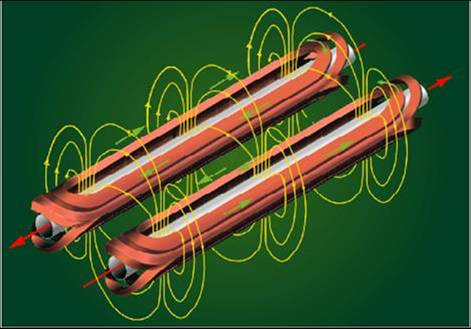
\includegraphics[width=0.65\textwidth]{dipole_1.jpg}\\
\vspace{0.5cm}
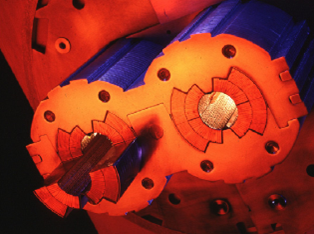
\includegraphics[width=0.65\textwidth]{dipole_2.png}
\caption[LHC dipoles]{LHC dipole magnets. Top: two dipole coils and magnetic field lines. Bottom: two beam pipes with the coils inside of the dipole magnet. }
\label{dipoles_coils}
\end{figure}



A  dipole magnet  must  be  curved to help a chain of dipoles complete 360 degrees. The curvature is 5.1 $mrad$ per dipole, which is equivalent to a  sagitta of  about  9 mm, corresponding to a radius of curvature of 2812.36 m.


The other important set of magnets is quadrupoles. They are used to ensure the proper beam dynamics. In total 392 quadrupole magnets ranging from 5 to 7 metres in length are used to squeeze the beam in transverse direction and to keep it narrow during the run duration. Additional special quadrupole magnets (SQM) are installed right before the IPs to focus the beams even more. That increases the density of protons in the beam and guarantees the maximum luminosity. In addition, SQMs help to decrease the chance of the parasitic collisions when bunches from the same beam or bunches outside of the IP centre interact (see Fig. \ref{quadrupoles}). To further correct the beam path (orbit), about 5000 higher order correcting magnets are used, which are evenly spaced around the circular trajectory of the LHC. 


\begin{figure}[H]
\centering
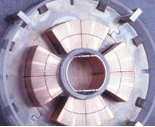
\includegraphics[width=0.4\textwidth]{quad_2.png}
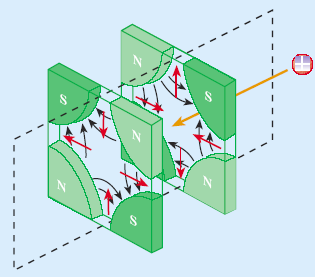
\includegraphics[width=0.37\textwidth]{quad_1.png}\\
\vspace{0.5cm}
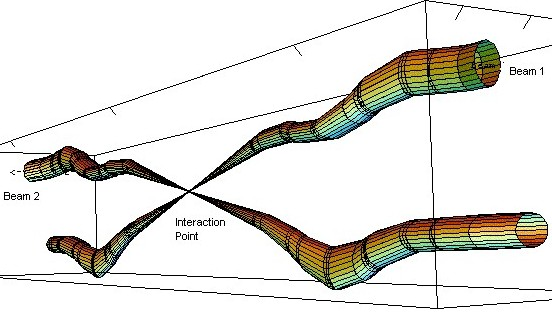
\includegraphics[width=0.7\textwidth]{quad_3.jpg}
\caption[LHC quadrupoles]{LHC quadrupoles. Top left: the coil of the quadrupole magnet. Top right: schematic view of the magnetic fields in the quadrupole. Bottom: two beams and the IP.}
\label{quadrupoles}
\end{figure}


To power the LHC, 1612 electrical circuits are used. Mostly these circuits are needed to power the dipole and quadrupole magnets, which is done in eight evenly spaced location of the LHC. A total of 3286 current leads are needed to connect all the circuits and power cables. More than a thousand of the leads operate between 600 A and 13 kA (see Fig. \ref{13kA_lead}). The other leads operate in the range 60 to 120 A. 

\begin{figure}[H]
  \centering
  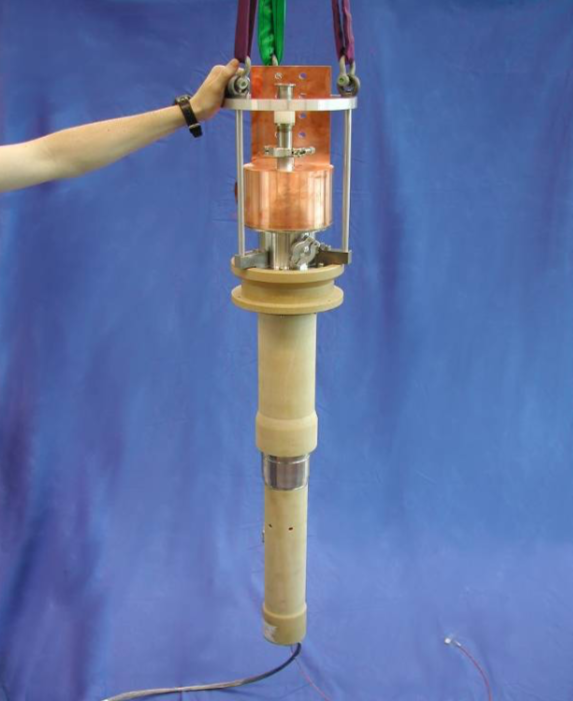
\includegraphics[width=0.5\textwidth]{13kA_lead}
  \caption{13 kA high-temperature superconducting current lead.}\label{13kA_lead}
\end{figure}


%%%%%%%%%%%%%%%%%%%%%%%%%%%%%%%%%%%%%%%%%%%%%%%%%

\subsubsection{Cooling System}\label{sec:cryogenic}

To ensure that dipoles are in the superconducting state, they have to be cooled to 1.9 K using superfluid helium-4. 

The cooling (cryogen) system is needed to keep superconducting LHC magnets at the appropriate temperature. The choice of the cooling gas depends on the magnet type and location. This dictates the required range of temperatures, which differs from system to system by 75 K. The cryogen system uses layered design with the temperature becoming progressively colder going from outside the dipoles closer to the beam pipe. 

The "coldest" part of the cryogen system is designed for the inner part of the dipoles. This system (see Fig. \ref{cryo_T_scale}) must cool down 37 Mkg of the LHC magnets within 15 days to the required temperatures, which is done through the system of pipes that transport the flow of the superfluid helium. The cryogen system must also be able to deal with the fast increases of the pressure flow and flow surges, as it is crucial for the LHC operation to keep dipoles constantly cooled and at the superconducting state.


The LHC tunnel is inclined in the horizontal plane by 1.41$^\circ$. This translates to 120 m difference in the vertical location of two diametrically opposite points of the tunnel with respect to the surface level and results in the additional hydrostatic pressure that can affect the flow of helium. This has been an important concern during the design of the cryogen system.


Since the cost to cool the LHC parts to 1.8-1.9 K temperatures is high, several temperature levels are employed (see Fig. \ref{cryo_T_scale}):
 
\begin{itemize}
\item 50 to 75 K for the thermal shielding used in the dipoles,
\item 20 to 300 K for upper ("warm") sections of the high-temperature superconducting current leads,
\item 4.6 to 20 K for lower temperature interception,
\item 4.5 K for radio frequency cavities and lower ("cold") sections of the high-temperature superconducting current leads,
\item 4 K for the transportation system that directs the 1.8 K helium to dipoles,
\item 1.9 K for helium in the superfluid state to cool magnet masses.
\end{itemize}

\begin{figure}[H]
  \centering
  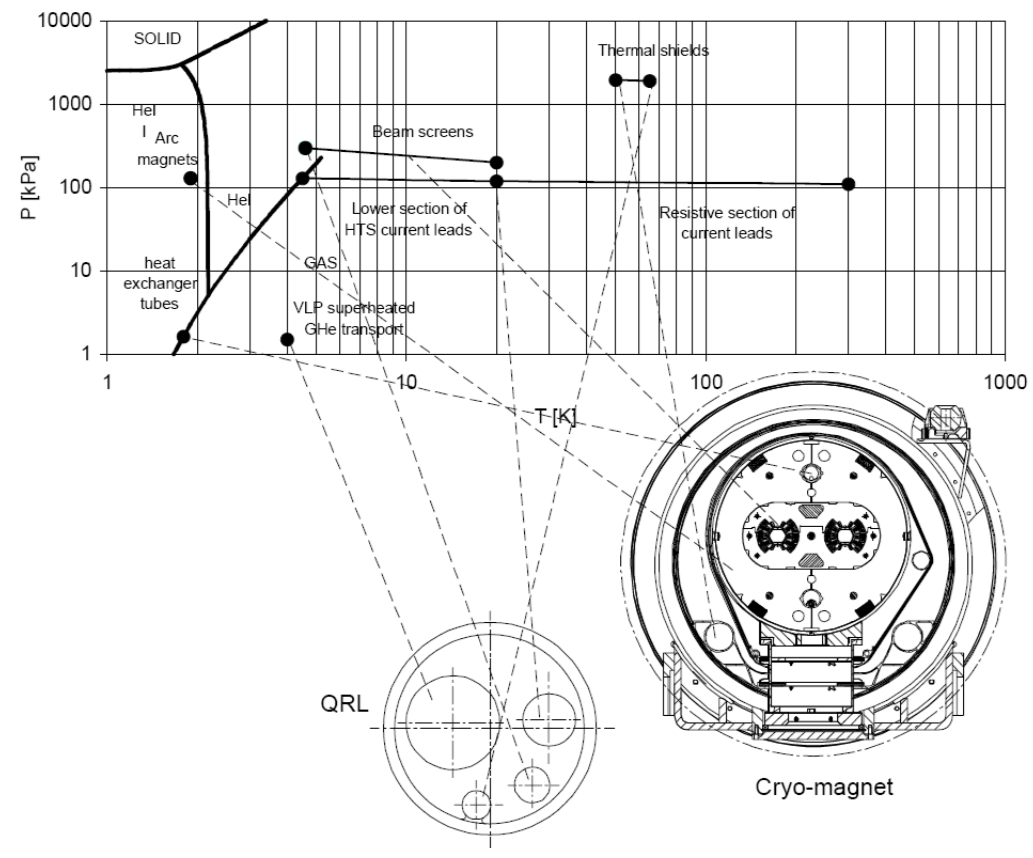
\includegraphics[width=0.7\textwidth]{cryo_T_scale}
  \caption{LHC cryogenic states and the temperature scale.}\label{cryo_T_scale}
  \label{cryo_T_scale}
\end{figure}


%%%%%%%%%%%%%%%%%%%%%%%%%%%%%%%%%%%%%%%%%%%%%%%%%


\subsubsection{Radio Frequency Cavities}\label{sec:rf}


Proton bunches need to be ramped to 7.5 TeV energies. To achieve this 13 TeV COM energy, eight superconducting radio-frequency cavities (RFC) are used per beam. They are located in front of the IPs of four experiments. Electromagnetic waves of 400 MHz with a peak field strength of 5.5 MV/m adjust the speed of protons in bunches. Each RFC (see Fig. \ref{lhc_rfc}) increases the energy of protons by 60 keV per revolution and it takes $O(20)$ minutes to reach 6.5 TeV beam energy. The RFC frequencies are increased gradually by 1 kHz to match the speed up of protons in the bunch as they gain more energy. When the ramp is completed, the RFCs are used to compensate for small energy losses due to the synchrotron radiation (7 keV per revolution). 




\begin{figure}[H]
\centering
%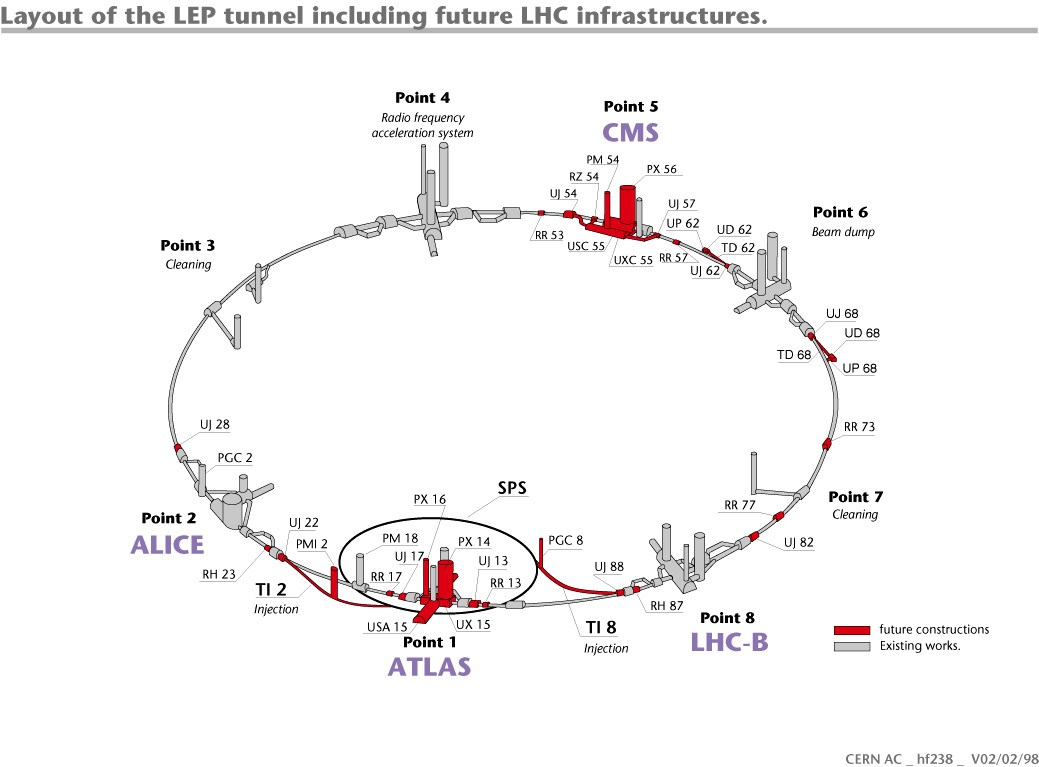
\includegraphics[scale=0.6]{lep}
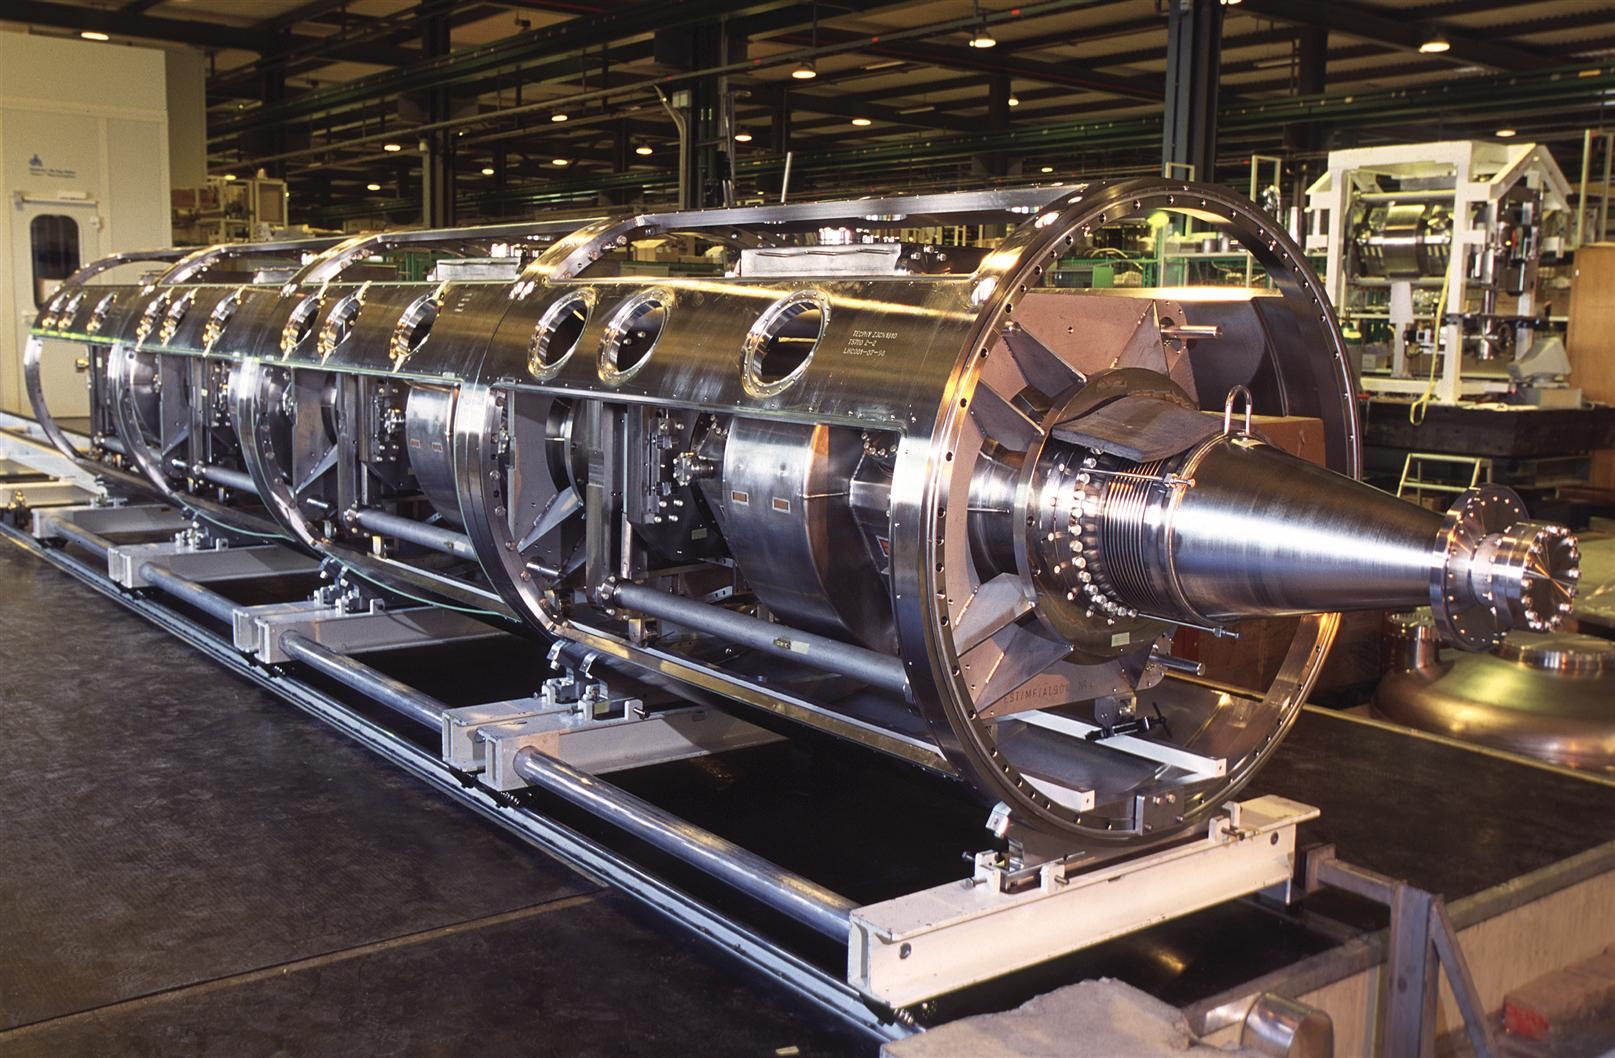
\includegraphics[width=7cm,height=4.2cm]{lhc_rfc}
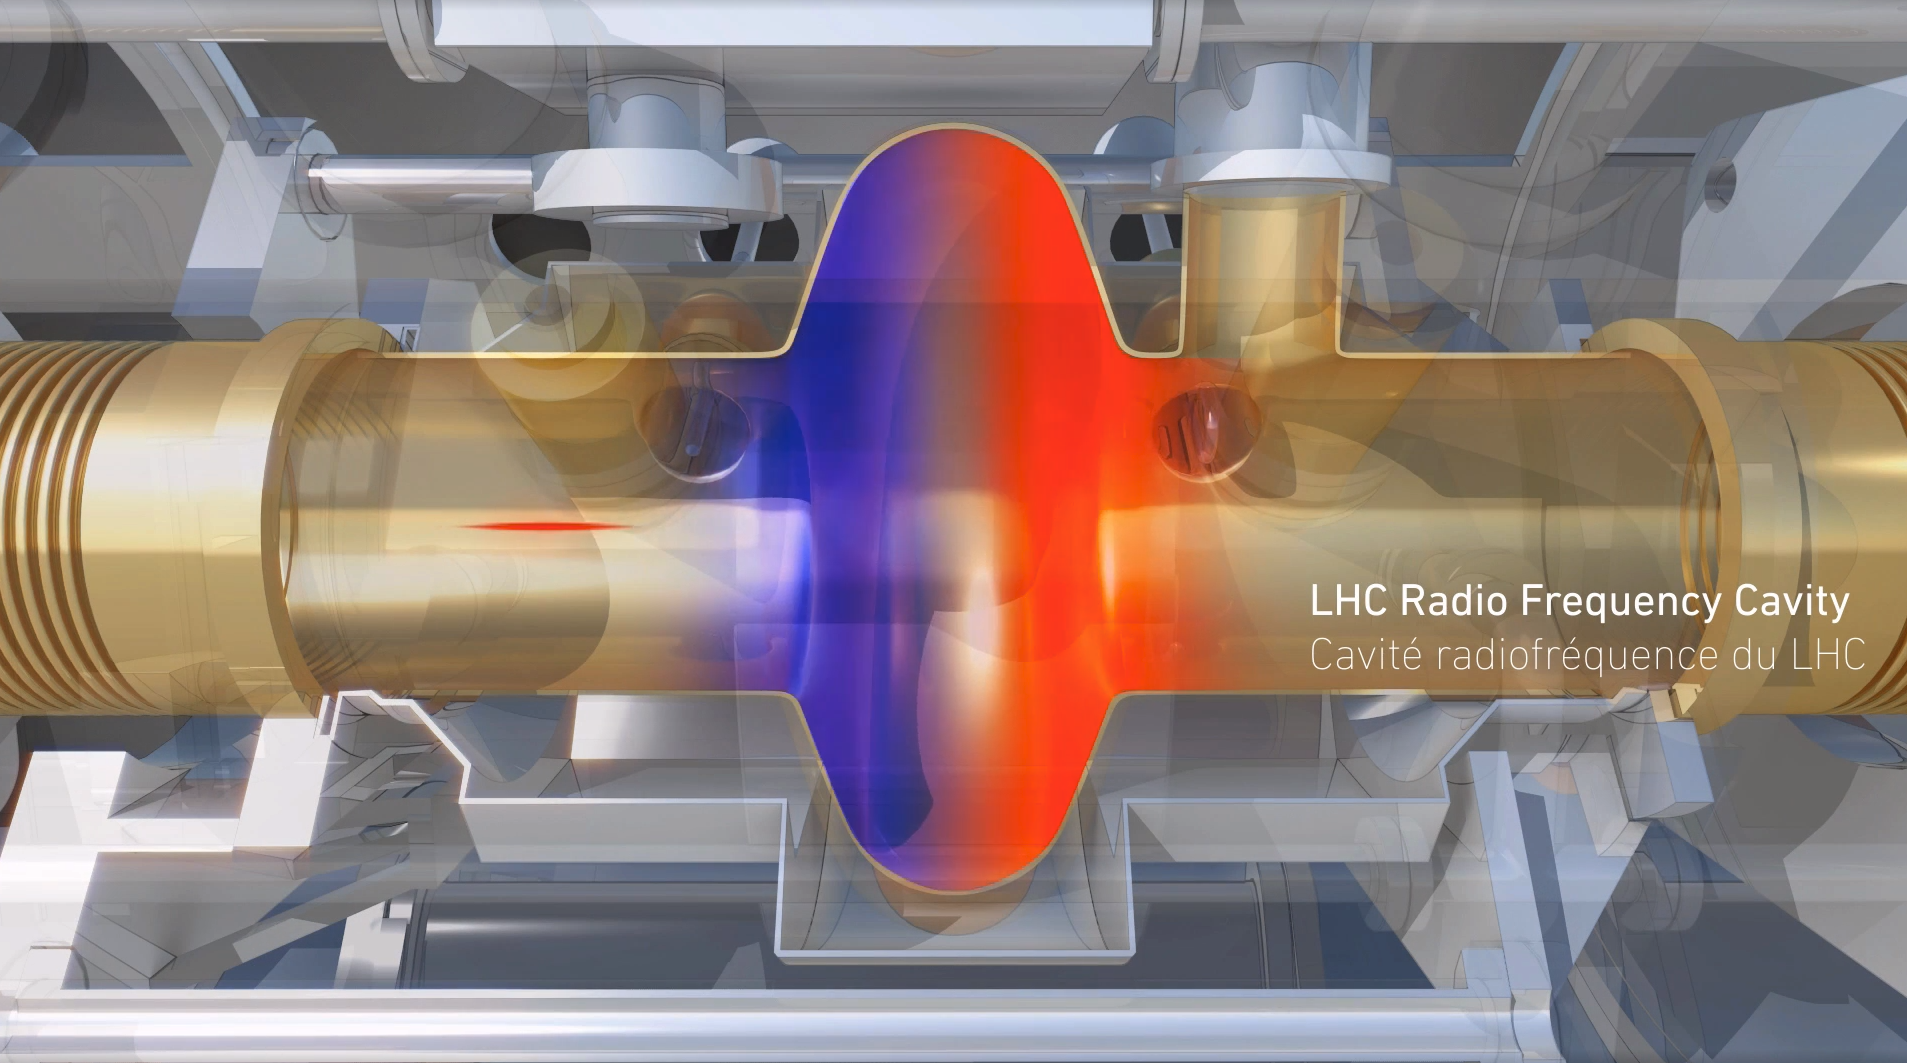
\includegraphics[scale=0.15]{rfc_lhc}
\caption[RF cavities module.]{LHC RF cavities. Left: a cryomodule with four RF cavities. Right: a schematic drawing of a single RF cavity. The colour field is used to denote Positive (red) and Negative (blue) polarities. A narrow beam traversing the cavity is shown in red. }
\label{lhc_rfc}
\end{figure}


%%%%%%%%%%%%%%%%%%%%%%%%%%%%%%%%%%%%%%%%%%%%%%%%%


\subsubsection{Vacuum System}\label{sec:vacuum}



The work of the LHC depends on three vacuum systems \cite{LHC_vacuum}. Without them, dipoles will not be at the superfluid state, the beams will not be able to circulate, and no stable collisions would be taken. With a total of 104 kilometres of vacuum pipes, the LHC owns the largest vacuum system in the world. The main types of vacuum systems are:

\begin{itemize}
\item insulation vacuum for cryomagnets,
\item insulation vacuum for the helium distribution line,
\item beam vacuum.
\end{itemize}


The insulation vacuum is needed to ensure the operations at both low temperatures of the magnets and the room temperatures in the tunnel. The insulation vacuum of $10^{-6}$ mbar is used for a total of 15000 cubic metres. To build this vacuum system, the LHC used 250,000 welded joints and 18,000 vacuum seals. 


The vacuum for the helium distribution lines is needed to protect from the heat the flow of the helium-4. This helium flow is used to cool down the dipole mass. Cryogenic distribution lines (QRL) of 3.3 km each are connected to eight cryogenic plants that pump the helium-4 into the LHC. The vacuum in these systems is at $10^{-7}-10^{-10}$ mbar level. 



For the beam pipes the LHC uses ultra-high vacuum of $10^{-10}$ mbar at cryogenic temperature of 5 K with the vacuum getting progressively closer to $10^{-11}$ mbar near the IPs, because in these locations collisions take place and any additional gas is highly undesirable. This vacuum is the emptiest space in the Solar System. This ultra-high vacuum is needed to reduce the beam degradation due to the beam-gas interactions in the pipe and parasitic collisions of bunches with the collimators near the IPs. 

Vacuum system are affected by the heat produced from the synchrotron radiation emitted by the proton beams when they are bent. To reduce the amount of this heat and to narrow down the beam size in the transverse direction when the beam widens, the LHC uses "beam screens", which operate between 5 and 20 K. 


\begin{figure}[H]
  \centering
  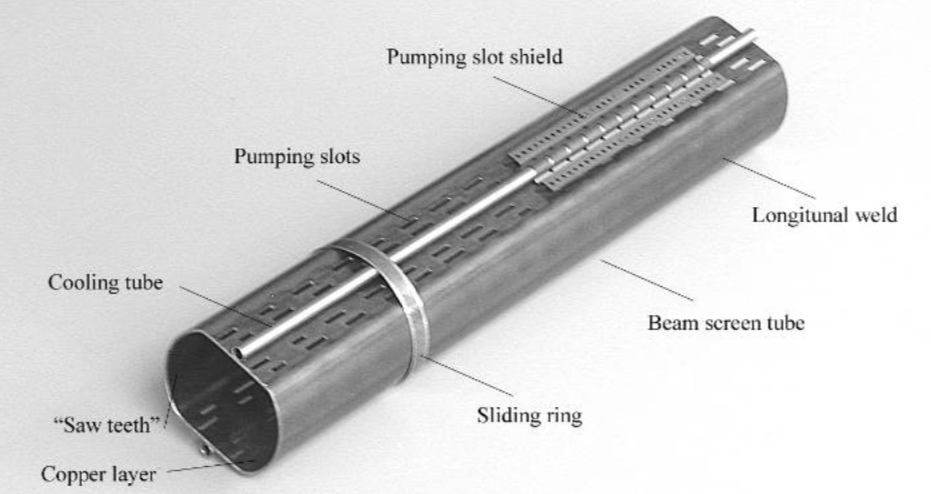
\includegraphics[width=0.7\textwidth]{beam_screen}
  \caption{Beam screen.}\label{beam_screen}
\end{figure}



The beam screens are necessary to reduce the number of protons scattering on the residual gas of the beam pipes, which could lead to a magnet quench and even interrupt the machine operation. The table below summarises the main heat sources that degrade the vacuum quality in the beam pipe, where the vacuum must exist at 1.9 K:


\begin{itemize}
\item synchrotron radiation (0.2 $W/m$ per beam),
\item energy loss by nuclear scattering (30 $mW/m$ per beam),
\item image currents (0.2 $W/m$ per beam),
\item electron cloud related effects (vary).
\end{itemize}



Now, that we discussed the LHC collider, we can continue with one of the main LHC detectors - the CMS detector - the one that was used to collect the data analysed in this thesis. 

%%%%%%%%%%%%%%%%%%%%%%%%%%%%%%%%%%%%%%%%%%%%%%%%%


\section{The CMS experiment}

                

The Compact Muon Solenoid (CMS) is a multi-purpose particle detector built to study a variety of complex particle interactions produced by the LHC. CMS is located in the underground cavern at the "Point 5", which is one of the four main IPs of the LHC. The CMS detector with the additional computing infrastructure is able to detect the produced particles, measure their main physics parameters, and to send the related data to computing data centres for persistent storage. 


The CMS detector has a cylindrical shape and consists of a central ("barrel") and two forward ("endcaps") sections (see Fig. \ref{CMS_detector}). 
CMS is the heaviest detector ever built with the mass of nearly 12500 tons. The mass is explained by the amount of the used superconducting metal, which serves as the magnet. The CMS is 21.6 m long and 14.6 m high. The CMS has an onion-like structure of concentric layer of detectors around the IP. In addition, at the outer part it has a large superconducting solenoid to produce inside the detector a homogeneous magnetic field of 3.8 T.

\begin{figure}[H]
  \centering
  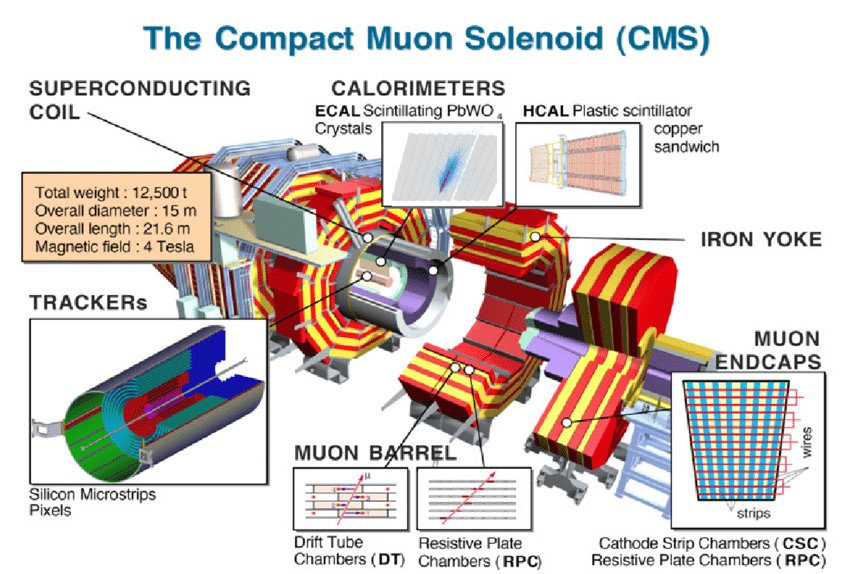
\includegraphics[width=0.8\textwidth]{CMS_detector}\\
  \vspace{1cm}
  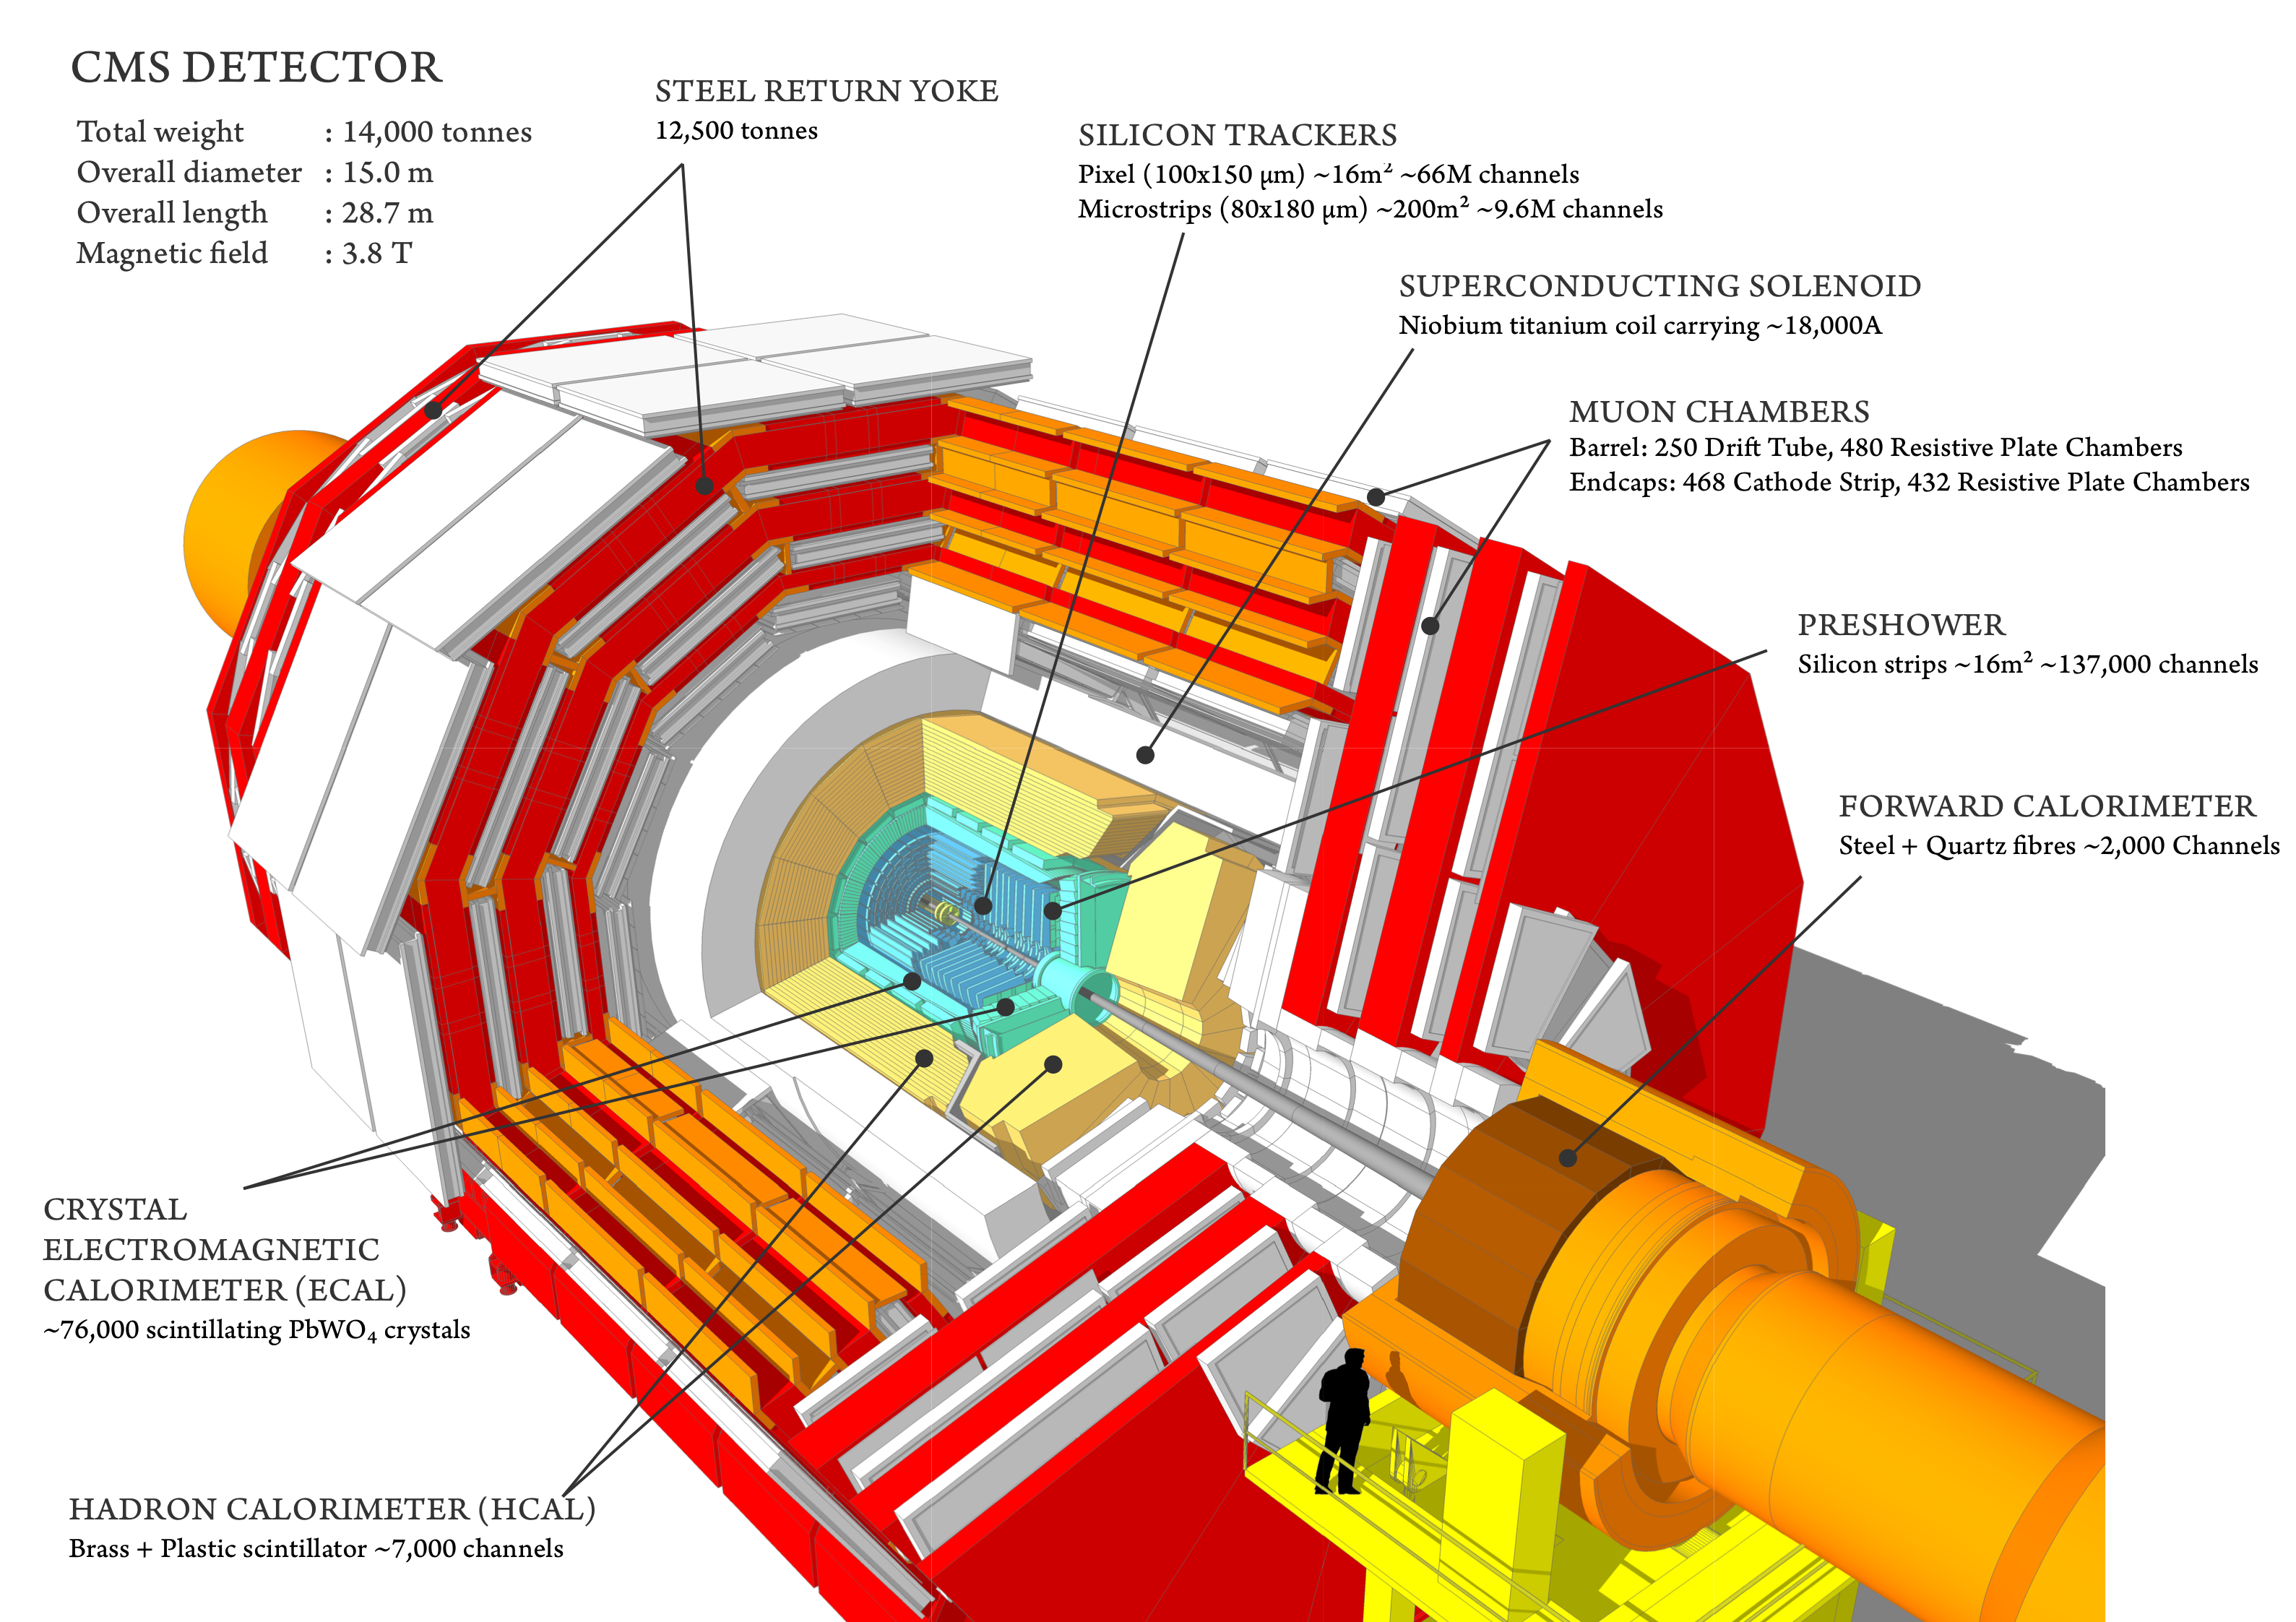
\includegraphics[width=0.8\textwidth]{cms_cross_section}
  \caption{CMS experiment with the main sub-detectors.}
  \label{CMS_detector}
\end{figure}


All sub-detectors can be categorised into trackers and calorimeters \cite{Hauptman:2011zza}. As the particle passes through the material of the tracker, it leaves a "track", which is a path of the emerging particle. Trackers focus on the direction and the track curvature of the charged particles. Tracking information allows the determination of the particle's momentum. 

There are two trackers in CMS: an inner tracking system that encloses the IP and the outer tracking system that is located outside of the solenoid magnet. The first system contains the Pixel and the Strip trackers. The second tracking system is dedicated for the muon detection and is usually called a muon tracker or a muon system. This system is embedded within a steel yoke of the magnet. The magnet yoke is made of five barrel wheels. Such an arrangement saves the CMS some space and also is used for the magnetic flux return. Additionally, it serves as a support for the embedded muon system, which is located outside of the ECAL and HCAL systems. Muons are energetic enough to traverse the ECAL and leave the detector. This muon system-magnet yoke structure provides a return field of the magnet of about 2 T and is used to measure the momentum of muons. This "two-directional" magnetic field with respect to the magnetic yoke, causes the muons trajectories to be bent in opposite directions in the inner tracker in contrast to the outer tracker. This important feature of the CMS detector is depicted in the CMS logo (see Fig. \ref{cms_logo}). 

\begin{figure}[H]
  \centering
  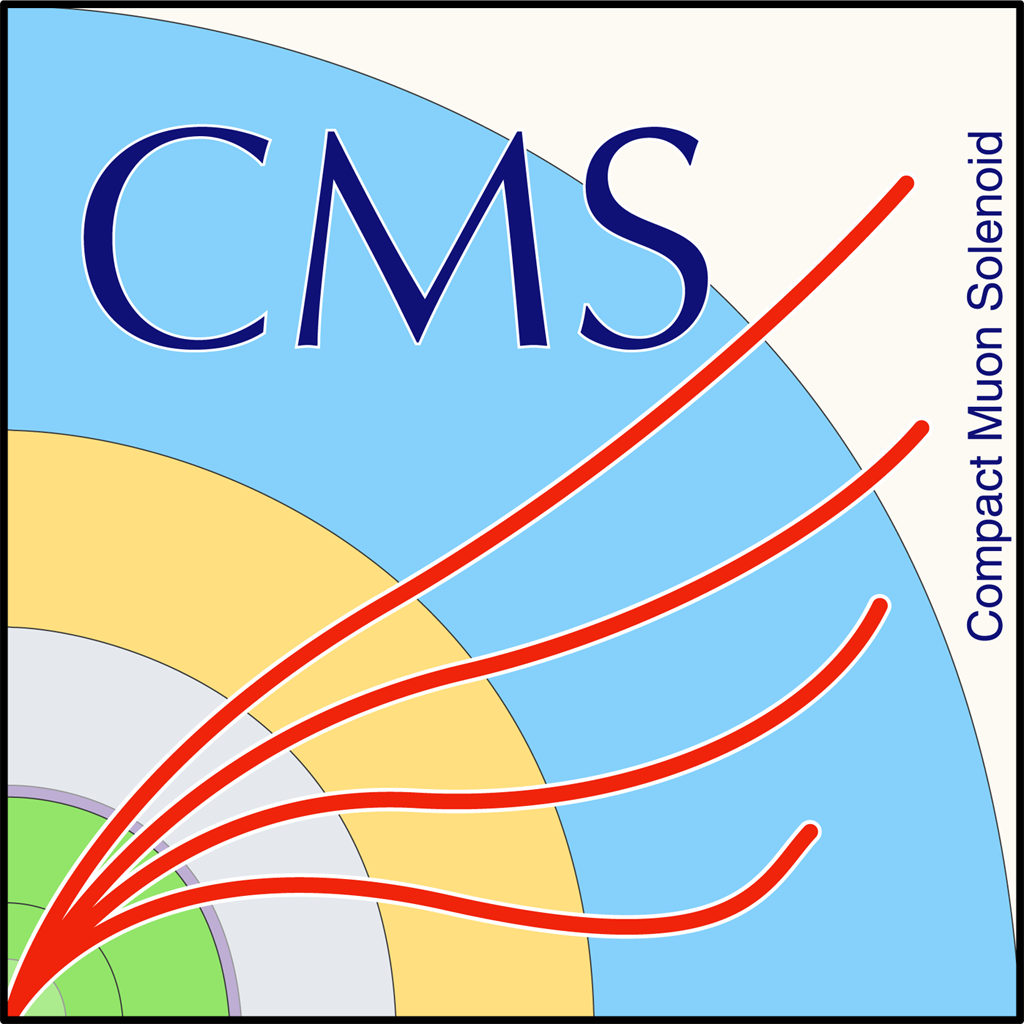
\includegraphics[width=0.4\textwidth]{cms_logo}
  \caption{The logo of the CMS experiment that is showing curved trajectories of the emerging muons.}
  \label{cms_logo}
\end{figure}


The CMS has two calorimeters: the electromagnetic and the hadronic calorimeters. They both rely on high density materials either to sample or to contain almost all the energy of the incoming particles with their secondary interaction products. However, these two systems focus on two different sets of particles. As will be discussed later, electromagnetic calorimeter (ECAL) is dedicated to measuring the energy of photons and electrons, while the hadronic calorimeter is targeting the measurement of the energy of hadrons.

Lastly, the rate of the incoming data is 40 MHz. This corresponds to almost 70 TB produced every second. This much data is impossible to store, and, most importantly, most of the information in this data is not interesting for future physics analyses. To reduce the data rate, the CMS uses a highly efficient system of triggers. The first one, the Level-1 (L1) trigger, reduces the nominal collision rate of 40 MHz to 100 kHz. The subsequent High-Level Trigger (HLT) further decreases the rate to 1 kHz. With the help of the trigger system, the original 40 TB per second rate is transformed into manageable 1 GB per second that is stored for offline analysis use. 

%%%%%%%%%%%%%%%%%%%%%%%%%%%%%%%%%%%%%%%%%%%%%%%%%


\subsection{The CMS coordinate system}

The CMS uses a a right-handed Cartesian coordinate system to define the axes of the colliding beams (see Fig. \ref{coord}). The centre is located at the IP and the x axis points to the centre of the LHC ring. The y axis points upwards, and the z axis points along the proton beam direction. Since the CMS detector has a cylindrical shape, the polar system is used in the x-y plane: a standard set of the azimuthal angle $\varphi$ and the radial coordinate $r$. The polar angle $\theta$ is defined in the r-z plane and a widely used in this thesis angular variable $\eta$ (called pseudorapidity) is defined as $\eta = \ln \tan(\theta/2) = \ln (\frac{\mid \vec{p}\mid + p_z}{\mid \vec{p}\mid - p_z})$. Additionally, a popular quantity in the collider physics - the rapidity - which is a function of the energy E and longitudinal momentum $p_z$ of the particle (the projection of $\vec{p}$ on the z axis), is given by $y = 1/2 \ln ( \frac{E + p_z}{E - p_z})$. Note that $\eta$ converges to $y$ when the mass is negligible and the particle travels with the speed close to the speed of light. Most angular variables that are used currently in the modern high-energy physics (HEP) are defined in terms of $\eta$ and $\varphi$:

$ \Delta R = \sqrt{(\Delta \eta)^2 + (\Delta \varphi)^2}$, with $\Delta \eta$ and $\Delta \varphi$ being the absolute values of the relative differences of $\eta's$ and $\varphi 's$ of two particles. 

Another extremely useful quantity is the projection of the momentum of a particle on the transverse plane. This variation of the momentum is independent of the z axis, hence, from the Lorentz boost, and is called "transverse momentum" $p_T$.  Similarly, the "transverse energy" of a particle is defined as $E_T = \sqrt{m + p_T }$. 


\begin{figure}[H]
  \centering
  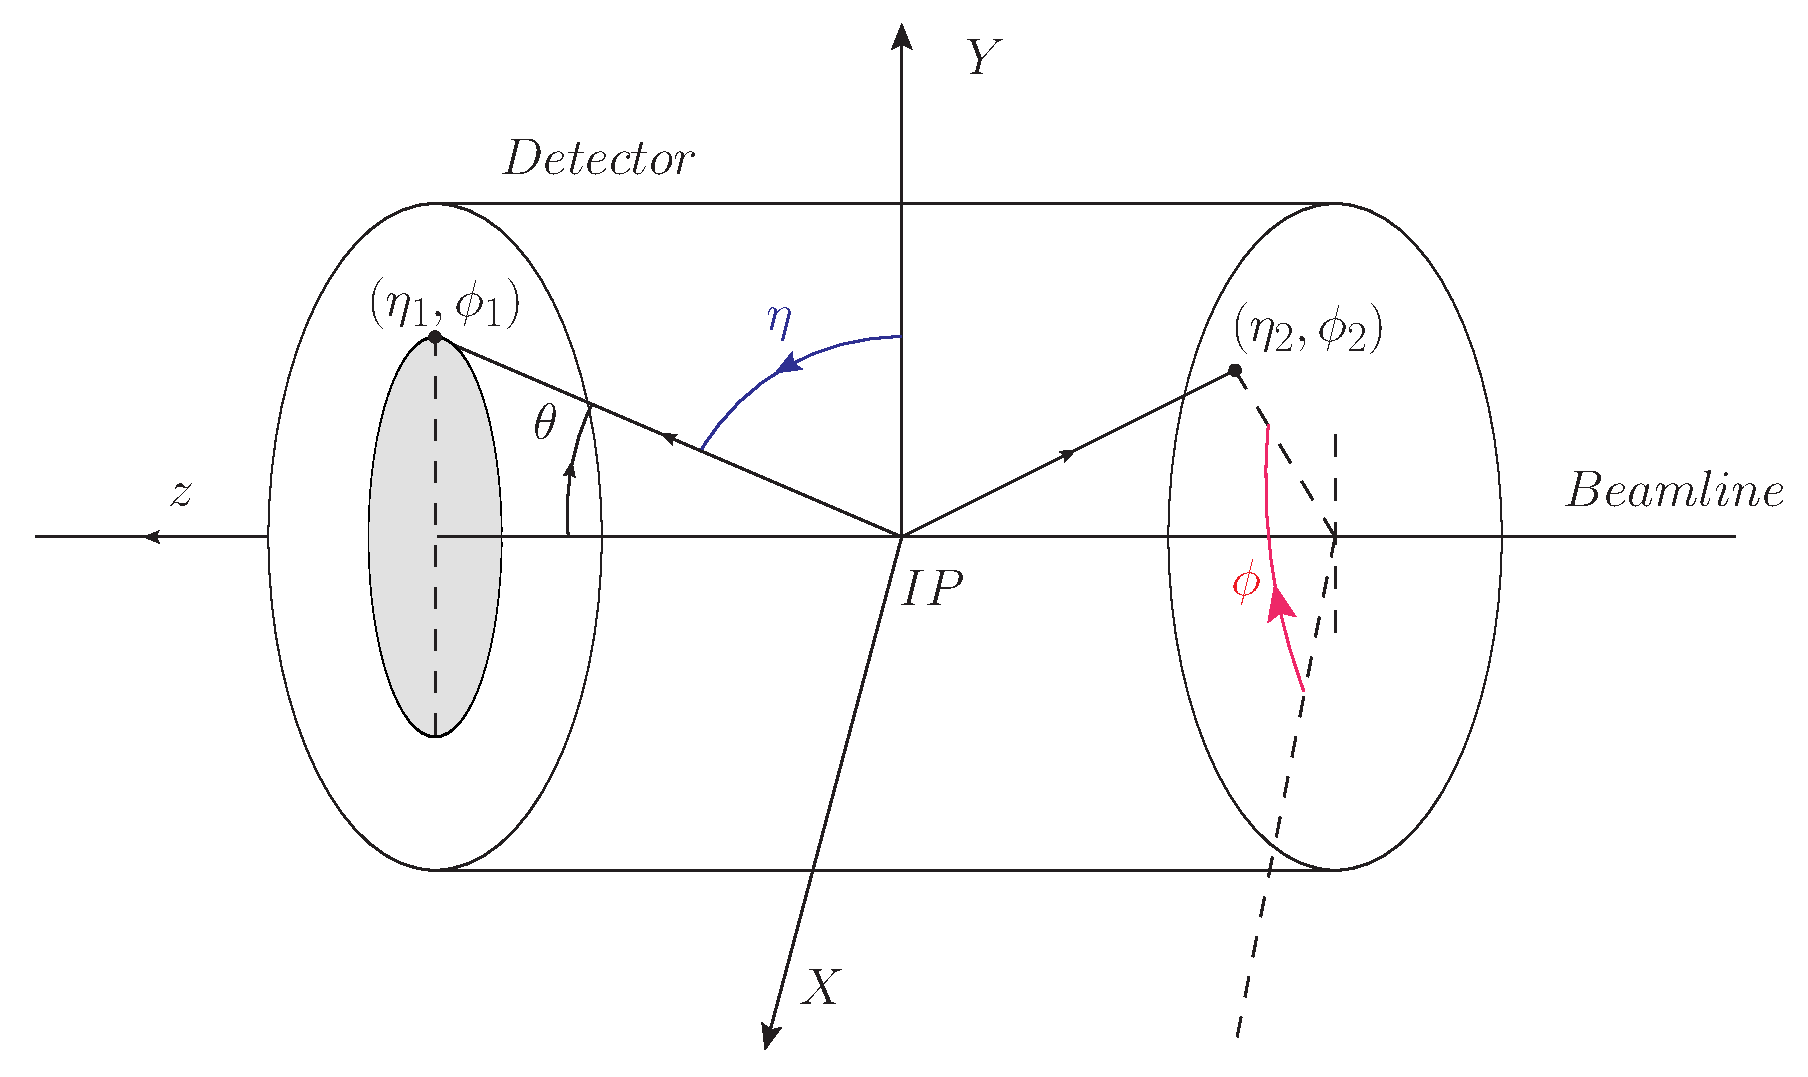
\includegraphics[scale=0.4]{coord}
  \caption[Coordinate system of the CMS detector]{Coordinate system of the CMS detector \ref{MonroyMontanez:2639240}.}
  \label{coord}
\end{figure}

%%%%%%%%%%%%%%%%%%%%%%%%%%%%%%%%%%%%%%%%%%%%%%%%%

\subsection{The Inner Tracker}

The inner tracker \cite{Tracker_phase2} (see Fig. \ref{inner_tracker}) is the closest subdetector to the IP. Using the tracker the experiment measures the trajectories of charged particles and reconstructs decay vertices. Since this system is constantly under the radiation coming from the interactions with the particle flux of nearly 100 MHz/cm at r =?? 4 cm, the design of the tracker focused on two main requirements: high granularity for precise determination of the vertices and tracks, and robustness against the radiation-hard environment with the operational time of at least 10 years. As a solution to both challenges, the CMS relies on the silicon technology that provides the tracker with the large surface of thin but highly granular active detectors. The tracking system has a diameter of 2.5 m and a length of 5.8 m covering the detector space of $|\eta|< 2.5$. 

The inner most part of the tracker - the Pixel detector ("Pixel")- consists of three layers in the barrel at the radii of?? 4.4 cm, 7.3 cm, and 10.2 cm. The Pixel also has two detector disks in forward regions. They are positioned 34.5 cm and 46.6 cm away from the IP. The Pixel is made of 1440 modules which contain 66 million pixel cells. Each cell is 100 by 150 $\mu$ m with 285 $\mu$ m thickness, which allows the determination of "hit" positions (the passage of the particle through the Pixel cells) in two directions z-$\varphi$ in the barrel and r-$\varphi$ in the endcaps.

The spatial resolution of each pixel about 10 $\mu$m in the r-? plane and 20 $\mu$m along the z direction. The spatial information that comes from the tracker is used to determine the main interaction point of the hard scattering ("the primary vertex") and also additional interaction vertices ("pileup"). Tracker also helps to reconstruct the displaced vertices ("the secondary vertices") of the particles that decay relatively fast, e.g., b-jets, which will be discussed later in this chapter. 

\begin{figure}[h!]
  \centering
  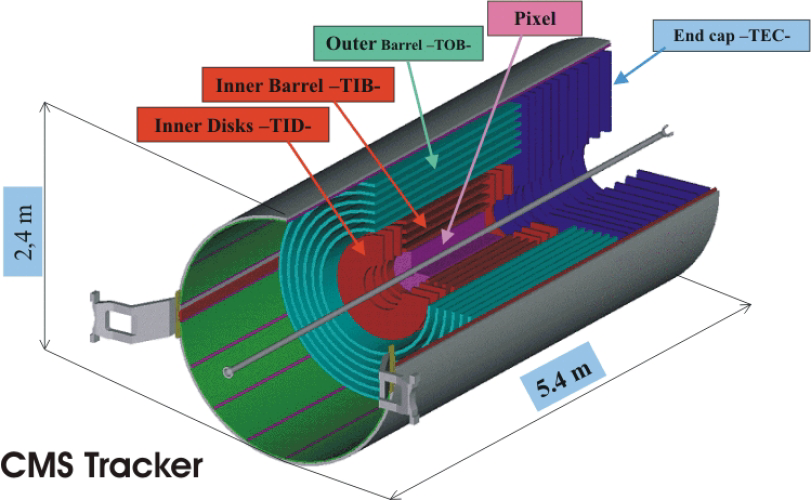
\includegraphics[scale=0.4]{inner_tracker}
  \caption[The inner tracker]{The inner tracker.}
  \label{inner_tracker}
\end{figure}


The outer part of the inner tracker is the strip tracker. It contains several subsystems and is made of almost 9.3 million strips arranged in different configurations in 15148 modules. The first subsystem is the tracker inner barrel (TIB), which consists of the four barrel layers of strip modules. The second subsystem is the tracker inner disks (TIDs), which is made of three disks of strip modules. Increasing the radius to about 60 cm, the tracker outer barrel (TOB) starts. TOB is made of six layers of strips. Finally, to cover high $\eta$ regions, the tracker endcaps (TECs) are used, which are made of two sets of nine disks of strips. 

Each strip is about O(20) cm long. Its thickness varies from 320 $\mu$m  for TIB and TID, to 320 $\mu$m - 500 $\mu$m  for TOB and TEC, respectively. Also width changes from 80 $\mu$m - 141 $\mu$m for TIB and TID, to 97 $\mu$m - 184 $\mu$m  for TOB and TEC, correspondingly. The resolution on the single point in the radial direction is 20 - 50 $\mu$m, and in the z direction it varries from 200 to 500 $\mu$m, depending on the value of r. 

All subsystems of the inner tracker have to be cooled down to about - 20$^{\circ}$.  This requirement is needed to minimise the damage of the tracker caused by the radiation from the collisions and to reduce overheating of the electronics. 

The material of the inner tracker has 0.4 to 1.8 radiation lengths (X$_0$), which corresponds to 0.1 to 0.5 nuclear interaction lengths ($\lambda_i $ ). Numbers vary with the $\eta$.



%%%%%%%%%%%%%%%%%%%%%%%%%%%%%%%%%%%%%%%%%%%%%%%%%


\subsection{The ECAL}


The inner tracker and the ECAL provide the detector with complementary measurements. The tracker focuses on the direction and the momentum of the particle and identifies only charged particles. The ECAL  \cite{ECAL_attendum} (see Fig. \ref{ecal2}), on the other hand, determines the energy of the particles and detects all particles that interact electro-magnetically, including photons and neutral pions. However, primarily the ECAL is designed to measure precisely the energy of electrons and photons. 

The ECAL is a highly granular detector that relies on the lead tungstate crystal (PbWO$_4$) technology. Electrons and photon passing through the crystal interact with its material and their energy is converted into the produced electromagnetic "shower". PbWO$_4$ crystals are known for being a popular choice of the scintillators: interactions with the crystal material produce the scintillation light that is further read out by the electronics. The PbWO$_4$ crystals have a high density (8.28g/cm$^3$), a small radiation length (X$_0 = 0.89$ cm), a short Moliere radius (R = 2.2 cm), and a fast response (80$\%$ of its scintillation light is produced within 25 ns). These characteristics are making PbWO$_4$ crystals ideal candidates for the ECAl, since they guarantee an excellent containment of the electromagnetic shower within the crystals. 

\begin{figure}[H]
  \centering
  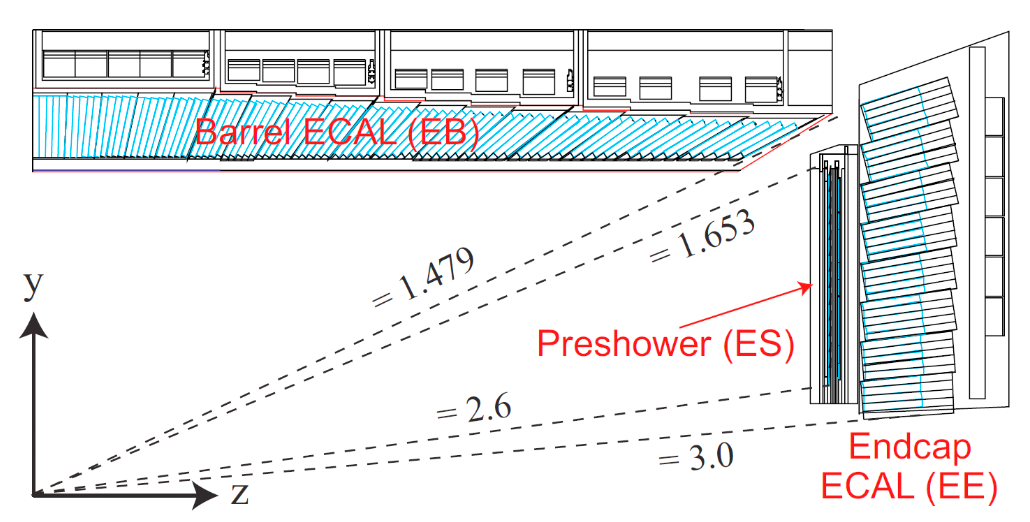
\includegraphics[scale=0.4]{ecal2}
  \caption[The ECAL]{The ECAL.}
  \label{ecal2}
\end{figure}

The ECAL has a barrel part (EB), covering the $|\eta|< 1.479$, and two endcaps (EE) covering 1.479 $< |\eta |  < 3.0$.
In the barrel ECAL is made of 61 200 crystals. Each crystal is 22 by 22 mm with a length of 23 cm. In the endcaps ECAL has 7324 crystals. There each crystal is 28.62 by 28.62 mm with a length of 22 cm. The crystals' layout is following a quasi-geometric projection with axes of crystals slightly tilted to ensure particle trajectories are never aligned with the intercrystal cracks. This layout is optimised for the best particle shower containment with respect to the position of the interaction point.  


The resolution of the ECAL is a function of energy of the incident particle E and can be decomposed into three terms. The first term is a stochastic term that is inversely proportional to the square root of the number N of scintillation photons produced in the interaction. In the main formula N is replaced by E, since N is proportional to E. The second term is a "noise" term that describes the noise in the detector.  The third term is related to detector imperfections and is represented by a constant fraction of E. The final dependence of the ECAL energy resolution $\sigma$ on the particle energy E is given by:

  
\begin{equation}
  \left(\frac{\sigma}{E}\right)^2 = \left(\frac{S}{\sqrt{E}}\right)^2 +
  \left(\frac{N}{E}\right)^2 + C^2
  \label{eq:ecal}
\end{equation}

From the dedicated calibration studies, the parameters in the formula above are found to be equal to: S = 2.8$\%$, N = 12$\%$, and C = 0.3$\%$. As a "standard" procedure, the CMS often optimises the performance of the subdetectors for 45 GeV electrons, since they correspond to a classical Drell-Yan decay of Z boson to two electrons. In this case, a typical energy resolution for 45 GeV electrons is about 2$\%$ in EB and 2-5$\%$ for EE. Near the Z peak (91 GeV), the constant terms dominates the resolution.


The ECAL is operated at a temperature of 18 $^{\circ}$ C and the "active width" of the ECAL material corresponds to 25 X$_0$. 

An additional subdetector, called the "Preshower", is installed right in front of the EE and covers 1.653 $ < | \eta |  < $ 2.6. The Preshower is designed to improve the discrimination of single photons from diphoton decays of neutral pions $\pi^0 \rightarrow \gamma \gamma$. This is a sampling calorimeter in which the material that produces the particle shower is distinct from the material that measures the deposited energy. Typically the two materials alternate. 
The Preshower has two lead layers which launch the electromagnetic showers. This "samples" the energy of the particles traversing the Preshower material.  After these layers, 2 mm-wide silicon strips are placed. They measure the deposited energy and transverse profile of the shower shape initiated by the lead layers. The "thickness" of the Preshower material corresponds to 3 X$_0$.

%%%%%%%%%%%%%%%%%%%%%%%%%%%%%%%%%%%%%%%%%%%%%%%%%


\subsection{The HCAL}

Hadrons normally go through the ECAL layers without being stopped. To absorb these particles, the HCAL \cite{HCAL_TDR} (see Fig. \ref{hcal2}) is placed around the ECAL. The HCAL focuses on particles that hadronise. This is a process of the formation of hadrons out of quarks and gluons. The HCAL detects with the charged and neutral hadrons such as pions, kaons, protons, and neutrons. Hadrons also produce collimated streams of secondary particles (jets) and these jets are identified by the HCAL. Additionally, the HCAL is used to measure indirectly the transverse energy of neutrinos, by the momentum imbalance technique, which will be discussed later in this chapter. 

The HCAL is split into HCAL barrel (HB) and HCAL endcap (HE) sections. They cover $ |\eta| < $1.3 and 1.3 $< |\eta| < $3.0 respectively. HB and HE are sampling calorimeters. They are made of a brass absorber and of active plastic scintillating tiles. The brass plates in HB have thickness of 56.5 mm and in HE the thickness if increased to 79 mm. The absorber material corresponds to 5.82 $\lambda_I$ at $\eta = 0$ to almost 10 $\lambda_I$ at $|\eta| < 1.3$.

The gaps in the absorber of the HCAL are filled with an active medium of 70000 plastic scintillator tiles. The scintillation light is guided by wavelength shifting fibres (WLSs) to hybrid photodiodes (HPDs). The scintillator is quite fast with the 68 $\%$ of the light been collected within 25 ns.

\begin{figure}[H]
  \centering
  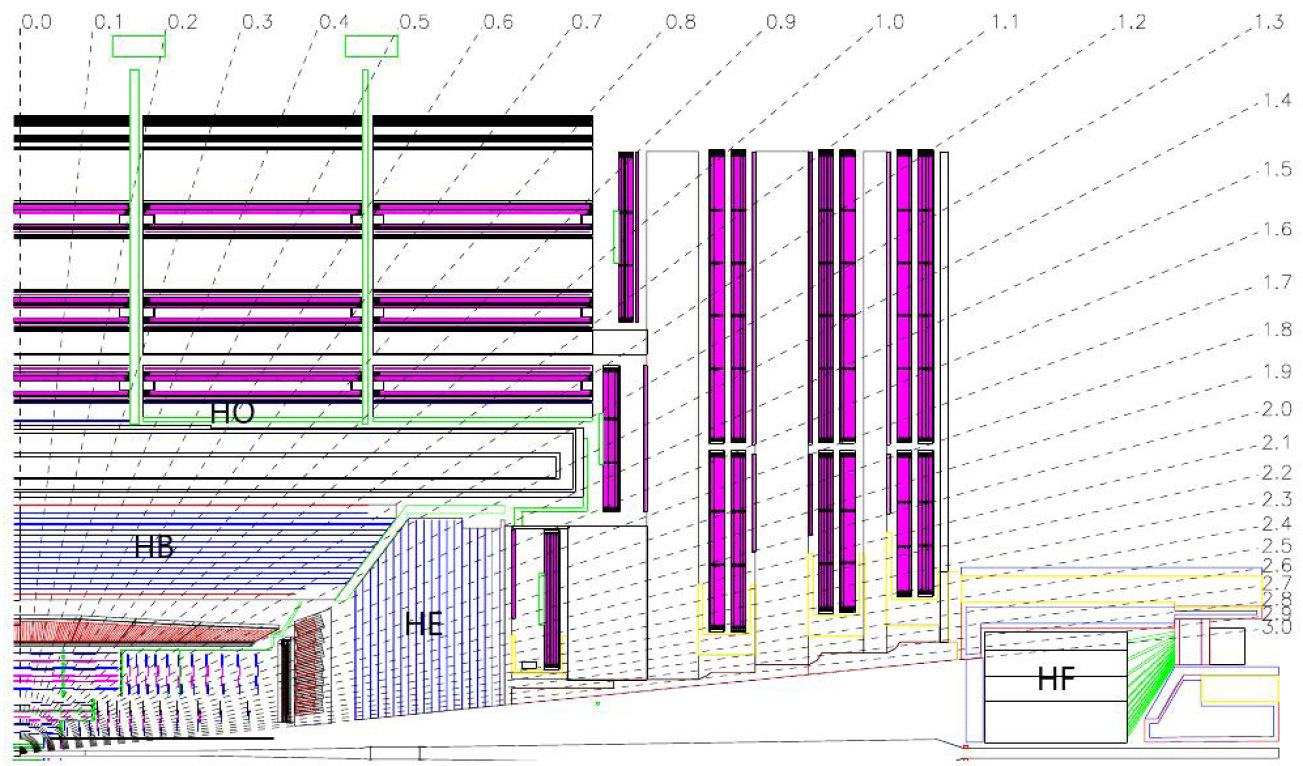
\includegraphics[scale=0.4]{hcal2}
  \caption[The HCAL]{The HCAL.}
  \label{hcal2}
\end{figure}


The CMS also has an outer calorimeter (HO) placed above the HB outside the solenoid. HO is called a tail catcher system and increases the total calorimeter thickness to 11.8 $\lambda_I$ in the barrel, with the magnet coil working as an extra absorption layer. The HO consists of five rings of scintillator tiles. A supplementary iron plate of 19.5 cm in thickness and a second layer of sensitive material are placed around $\eta =$ 0 to enhance the absorber depth there. 

In the forward directions, two forward calorimeters (HF) extend the coverage to  $|\eta| = 5.2$. The HF is composed of steel absorbers and quartz fibres that produce Cherenkov light when the particle in the material travels faster than the light in that medium. The light is further collected by photomultiplier tubes (PMTs). 


Since the HCAL is located between the ECAL and the internal surface of the solenoid, the space allocated for the HCAL is not enough for the HCAL to fully absorb the hadronic showers and this imperfect containment of the hadronic shower limits the performance of the HCAL. Comparing with the formula \ref{eq:ecal}, for the single pions the values are given by:  by S = 115 $\%$, N = 52  $\%$, and C = 5.5 $\%$ \ref{Baiatian:1049915}.


%%%%%%%%%%%%%%%%%%%%%%%%%%%%%%%%%%%%%%%%%%%%%%%%%



\subsection{The Superconding Solenoid}


The NbTi superconducting solenoid (see Fig. \ref{solenoid}) of 6 m in diameter is the core of the CMS experiment. The magnet operates at a temperature of 4.5K. The bulk of the CMS detector weight (90 $\%$) comes from the magnet steel return yoke and structural supports which together weigh 12500 tonnes.
 
 \begin{figure}[H]
  \centering
  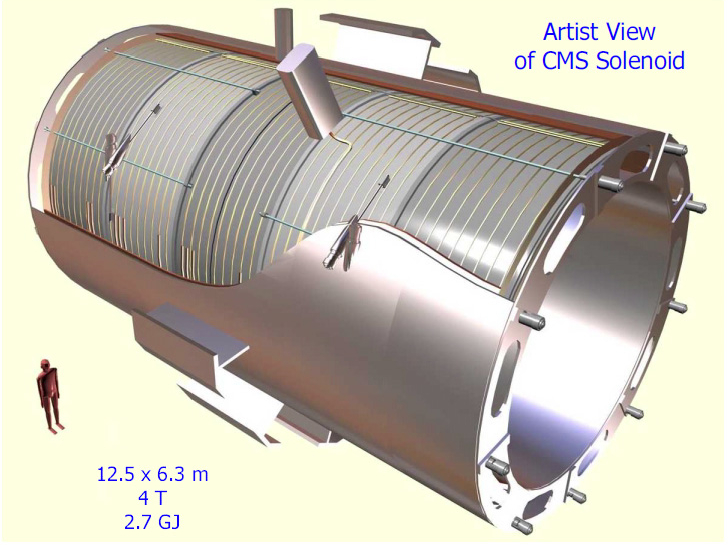
\includegraphics[scale=0.4]{solenoid}
  \caption[The CMS superconducting solenoid]{The CMS superconducting solenoid.}
  \label{solenoid}
\end{figure}

The solenoid is central part in the CMS detector design. The idea was to have a uniform magnetic field capable of bending the trajectories of charged particles as they traverse the detector. When a low energy particle is produced, it has a helical path and will be fully contained within the detector. On the other hand, when a highly energised particle is produced, the trajectory is seen as a "straight" incomplete arc. Both situations lead to imperfect measurement of the momentum. The primary measurements of the tracking system are presumed to be Gaussian distributed; but the momentum of the particle that the tracker measures is not Gaussian distributed. However, the sagitta is Gaussian distributed, and that is why widely used in the particle physics. 

When the particle in the magnetic field passes thorough the material of the detector, the path deviates from the ideal circular line due to random fluctuations and multiple scattering. The sagitta term is used to quantify the depth of the circular arc and is equal to the distance from the centre of the arc to the centre of its base. Since the sagitta is following a Gaussian distribution, it may be approximated by simpler expressions in many calculations of the momentum resolution. 

The magnetic field strength B and the length of the track L are dictated by the design of the detector. Since the momentum resolution is given by $\sigma_p / p^2 \approx \sigma_x / B L^2 $ (see \cite {Hauptman:2011zza}) and improves linearly with magnetic field B, this is the reason why the CMS decided to invest much of the detector space and budget in the magnet. For a track of the length of O(1) m in the magnetic field of O(3) T, the sagitta is equal to 1 mm, which can be measured very precisely. 


%%%%%%%%%%%%%%%%%%%%%%%%%%%%%%%%%%%%%%%%%%%%%%%%%

\subsection{The Muon Tracker}

Many physics analyses in the CMS rely on a precise measurements of the muons in the detector. Although muons are detected by the inner tracker, that information cannot be used by the trigger (will be discussed in the following subsection). Therefore, CMS has an outer tracker or muon tracker \cite{Muon_system_TDR} (see Fig. \ref{cms_muon_system}) located outside the calorimeters and the solenoid. Because of the typical muon energies, muons produced in collisions at the LHC traverse the detector material with the minimal energy losses. To measure energy of muons, the CMS uses the muon tracker, which relies on various gaseous detector technologies. The muon tracker is inserted into the gaps of the flux-return yoke. Tracks in the muon system are used to reconstruct standalone muons, and in combination with the inner tracker, to reconstruct the global muons.

 \begin{figure}[H]
  \centering
  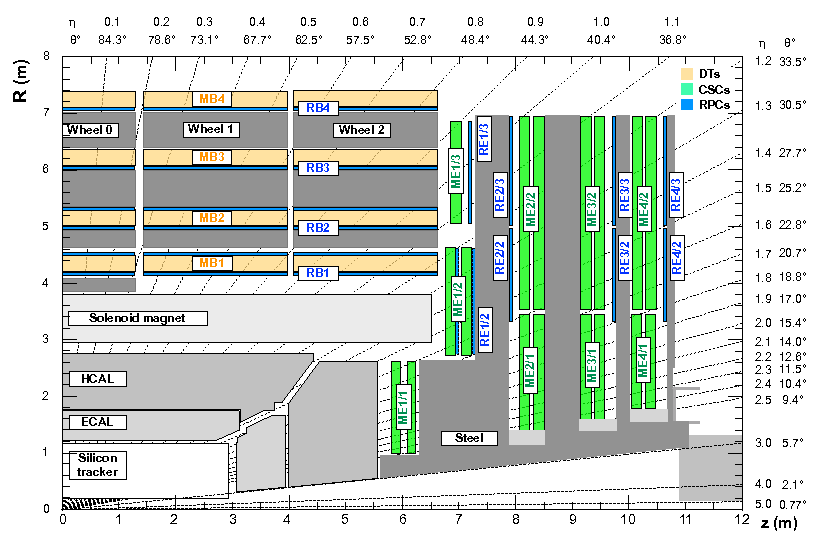
\includegraphics[scale=0.4]{cms_muon_system}
  \caption[The CMS muon tracker]{The CMS muon tracker.}
  \label{cms_muon_system}
\end{figure}

CMS muon system has three subdetectors: the drift tubes (DTs), the cathode strip chambers detectors (CSCs), and the resistive plate chambers (RPCs). In the barrel region, the CMS is equipped with the DT system, which is 250 drift tubes  arranged into five barrel section ("wheels"). Each wheel is made of four concentric rings of DT stations. The working elements of the DT system - cylindrical cells with the rectangular base of 4.2 by 1.3 cm$^2$ - are tubes with an anode wire in the the mix of argon and CO$_2$ gases. DT cells are 2.4 m long and are organised in three groups of four elements (three "super-layers"). When the muon passes through super-layers, it ionises the gas in the cells and released electrons start moving to anodes. Using the time it takes for electrons to reach the anodes, the muon position and direction can be determined. DT resolution of a single-cell hit positions ranges from 200 $\mu$m in the r-$\varphi$ plane to 200-600 $\mu$m for forward directions. 

CSCs are used in the forward direction to cover the region of 0.9 $ <|\eta|<$2.4. CSCs chambers are multi-wire chambers made of cells  that have a trapezoidal shape. Chambers contain radial copper cathode strips and, perpendicular to those, gold-plated tungsten anode wires. Each cell is filled with the mix of Argon, CO$_2$, and CF$_4$ gases. The strip cells have a single-layer resolution of 300-900 $\mu$m. A CSC chamber provides a spatial resolution of 40 -150 $\mu$m.


To improve the performance of DTs and CSCs, RPCs are used and are covering the barrel and endcaps in the range of $|\eta| <$ 1.9. 
RPCs are double-gap chambers consisting of two resistive 2 mm in thickness Bakelite layers separated by a 2 mm layers filled with a mix of C$_2$H$_2$F$_4$, $i$C$_4$H$_{10}$, and SF$_6$ gases.

RPCs operate in avalanche mode, producing an avalanche when the muon traverses the gas of the cell. RPCs have a spatial resolution of 0.8 - 1.2 cm, which is not as good as the ones provided by other muon subsystems, but RPCs have an advantage in terms of an excellent time resolution - just 3 ns. The barrel and the endcaps contain in total 10 RPC stations.



%%%%%%%%%%%%%%%%%%%%%%%%%%%%%%%%%%%%%%%%%%%%%%%%%%%%%%%%%%%%

\subsection{The Triggers and DAQ}

The CMS trigger \cite{Trigger} is a system responsible for selecting events of interest and storing them for the offline analysis. The trigger has two stages: the L1 trigger (see Fig. \ref{L1trigger}), which reduces the event rate from 40 MHz to 100 kHz, and the HLT trigger, which further decreases the rate to nearly 1 kHz. The L1 trigger consists of the custom hardware that processes a part of the information from calorimeters and outer tracker systems. The HLT trigger is a part of the detector readout system (DRS) and uses the full detector information for event reconstruction. The HLT is a computing farm consisting of 22000 CPU cores that produce a decision on whether to save or to skip the event in an average time of about 220 $\mu$s. DRS is integrated in the higher level data acquisition (DAQ) system \cite{DAQ}. The selected events are collected and sent by the DAQ to the tapes of the CERN Tier-0 for the persistent storage. 


L1 and HLT systems have differences and similarities. They operate at the different time scales and the volumes of data they are processing are completely different. However, the goals of these systems are the same - to identify and reconstruct physics objects and combine their properties to produce an acceptance/rejection decision for each event. 

%%%%%%%%%%%%%%%%%%%%%%%%%%%%%%%%%%%%%%%%%%%%%%%%%


\subsubsection{The L1 Trigger}


L1 system \cite{CMS_TDR} contains a "menu" of 500 algorithms or "seeds" designed to identify useful physics events. These menus include trigger criteria varying from basic single-object identification to complicated selections requiring some topological conditions to be met. Each seed has a set of assigned "Prescale" factors $f$ that reduce the rate of events accepted by a particular trigger algorithm from 100$\%$ to $100/f\%$. Prescale factors are necessary since the luminosity level decreases during the run period. They adjust the trigger rate to keep it constant during the data taking time. 

Since the processing time of the L1 system is very important for the whole CMS operation, the L1 is built using FPGAs and ASICs custom hardware. L1 produces decisions within 3.8 $\mu$s. Data from all the calorimeters is first processed by the L1 regional calorimeter trigger (RCT) and then by a more selective global calorimeter trigger (GCT). 

 \begin{figure}[H]
  \centering
  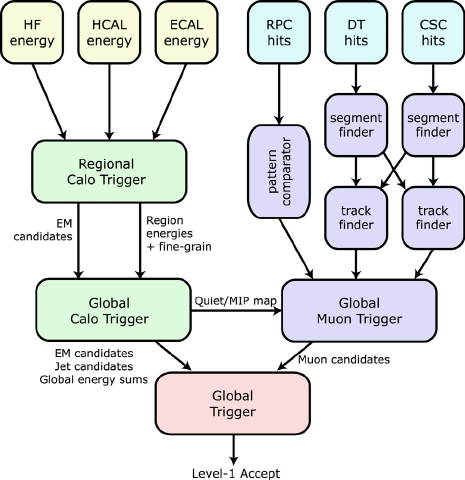
\includegraphics[scale=0.4]{L1trigger}
  \caption[The CMS L1 trigger layout]{The CMS L1 trigger layout.}
  \label{L1trigger}
\end{figure}

The RCT receives the information about energy deposits from all calorimeters and covers the range $|\eta|<$5. The RCT processes this information in parallel and produces e/$\gamma$ candidates as an output. The information from the inner tracker is not available, therefore, L1 identifies both electrons or photons, but cannot distinguish them. L1 also detects jets, taus, missing transverse energy (MET or \ETslash or \PTslash), and muons. L1 RCT is responsible for determining the first estimates of the several main parameters of interest: $p_T$, isolation (described later in this chapter), etc. 

First stage reconstruction uses particle "hits" in the muon detectors and analyses them using track finder algorithms. All three muon detectors of the CMS are used by the L1 muon trigger. Using DT and CSC systems, track segments from the hit information are identified. The pattern recognition algorithms are applied to these segments to reconstruct muon candidates and measure their momenta. 

More complex but slower algorithms then re-use hits for a more precise particle identification using a global muon trigger (GMT). 
The hits from the RPCs are used directly by the pattern comparator trigger (PACT) that reconstructs muon candidates at the high radii. Then several regional track finder algorithms sort the identified muon candidates and send this information to the GMT. Each candidate contains $p_T$ and angular information. 

The GMT then combines the muon information from different subsystems to avoid duplicating the candidates. The GMT also performs more tight track quality checks and may discard a portion of the input candidates it received. 

Finally, the information from the GCT and GMT is combined by a global trigger (GT). The GCT sorts the created e/$\gamma$ candidates, identifies jets, and calculates \ETslash. The final decision of the GT is to store or to skip the event. If the event satisfies the acceptance requirements and is going to be kept, the L1 accept signal (LAS) is generated and propagated by the trigger control and distribution system (TCDS) to all subdetectors. 


The GT is the final step of the CMS L1 trigger system and implements a menu of triggers. The output of this system is used as an input to the HLT algorithms. 

%%%%%%%%%%%%%%%%%%%%%%%%%%%%%%%%%%%%%%%%%%%%%%%%%


\subsubsection{The HLT Trigger}

The selection done by the HLT mimics the offline analysis - for all reconstructed objects in the event: electrons, muons, and jets - the identification criteria is applied to select only events of interest. What these events are each offline analysis defines in a different way, but to name a few, almost all analyses need true prompt leptons, well reconstructed jets, or some other commonly used objects. 


The HLT computing farm has the event filter farm, which consists of filter-builder units (FBU). In the FBU the parts of the events and information from different detector subsystems is combined to produce "complete" events. Then the filter unit unfolds the raw detector data into experiment specific data structure and performs the event reconstruction and trigger filtering. 


The whole event processing procedure of the HLT is centered around the HLT path. The HLT path is a set of algorithmic instructions that in a sequential manner reconstructs physics objects and performs the object selection. The complexity of the steps in the path sequence increases and the quality of the physics objects (the probability to have a correct label) improves too. After this step is completed, selected events are sent to another software processing farm. In this storage manager farm, the date is archived, stored locally on disk, and later sent to the CMS Tier-0 computing center for offline use. 

Most data enters the queue for processing and is ready to be sent to Tier-0 very soon. In some cases the special data, the "parked" data, may be collected and kept until the run is finished. In this situations the CMS tape is used and the data has a high-priority for "parking". This may include "hot topic" analyses such as vector boson fusion or parton distribution studies such as Drell-Yan process.

The output of the HLT is limited by capacities of the Tier-0. This includes the bandwidth of the data transfer as well as the amount of available tape. This complicates the work of the DAQ, since in addition to physics data streams, the calibration streams also need to be stored. These streams, though, use information only from few subdetectors. 


%%%%%%%%%%%%%%%%%%%%%%%%%%%%%%%%%%%%%%%%%%%%%%%%%

\subsubsection{The DAQ system}



The DAQ systems in the modern high energy physics are responsible for any tasks. The challenges are well known: high data rates and volumes, limited tape space and transfer bandwidth. CMS DAQ is based on the homogeneous architecture, scales well with the different beam energy regimes and data rates, and stable  performance  in  a  variety  of  operating  conditions.  

As an example of the complex computing task that is elegantly solved by the DAQ system, let us discuss the aforementioned FBUs system of the HLT. FBU relies on a single multi-core machine and the communications with other units are done via shared memory. The data from the full detector is used for the filtering process. Complicated offline-like reconstruction algorithms are then used for the full precision event selection. With more CPU cores available for the Run-2, the per-event time budget is increased to "comfortable" 175 ms per event, which is a long enough time to run most of the CMS reconstruction algorithms. 

The current CMS DAQ was developed to address these core requirements: 

\begin{itemize}
\item The data from one or several data transfer lines is available for other lines,
\item the event building is done in parallel profiting from multiple processing units,
\item almost real-time process monitoring,
\end{itemize}


Proper design patterns are used in the software for DAQ, which decouple the user  interface from the implementation. The design also allows for the remote control. The  software  system  can be run on a number of different  operating  systems  and  hardware  platforms.   The memory  management  tools  of  the  underlying  system  are not linked directly to the applications, it is done using a dedicated abstract addressing  scheme.

%%%%%%%%%%%%%%%%%%%%%%%%%%%%%%%%%%%%%%%%%%%%%%%%%
  
\subsection{The CMS design}

Now that we discussed all CMS subdetectors and DAQ, we can look back and summarise in one list what were the requirements on the design of the CMS detector to successfully complete its physics program. Here we refer to the CMS Technical Design Report \cite{CMS_TDR}: 


\begin{itemize}
\item good muon momentum resolution over the momentum scale covering almost a TeV range, good dimuon resolution (mostly $Z \rightarrow \mu \mu$ and $H \rightarrow \mu \mu$) at the O(100) GeV. The capability to determine correctly the charge of the highly energetic muon all the way up to 1 TeV. 
\item Good momentum resolution of all charged particles in the inner tracker.
\item Good diphoton mass resolution with the focus on the $H \rightarrow \gamma \gamma$ discovery channel. Also, the ability to reject $\pi^0 \rightarrow \gamma \gamma$, which is one of the main background processes to many physics analyses.  This requirement mostly concern the performance of the ECAL. 
\item Good resolution of the missing transverse energy (discussed in the section below) and of the mass of the two-jet system. This task depends heavily on the performance of the HCAL.
\end{itemize}

%%%%%%%%%%%%%%%%%%%%%%%%%%%%%%%%%%%%%%%%%%%%%%%%%


\section{The object reconstruction}\label{sec:cms_reconstruction}

  
  - somewhere a section on physics objects where you discuss that there are tracks, there are jets, there are b-jets, what it means an isolated lepton, what it means missing momentum, and so forth. For example, Ekaterina has a section on particle flow, if I remember right, where she discusses that. Or you can have a section that just discuses the proton-proton collisions environment and explains that many particles created in collisions are unstable and decay right away. What is observable in an experiment such as CMS is longer-lived or stable particles. These include electrons, muons, photons, and some ground state hadrons. At the same time, energetic quarks or gluons hadronize and can be seen in a particle detectors as jets of hadrons (so define jets here). Same for tau leptons, we detect them either as electrons/muons, or hadronic jets. Etc. If you have such a conceptual paragraph here, some time later you can have a particle flow discussion when it is time to be more specific. But discussion at this level above would allow you to then discuss the requirements on CMS design using terms like b-jets or isolated leptons.

  EGAMMA AT LEAST SAY THAT HAS BEEN WORKING AND SHOW SOME PLOTS?

\end{normalsize}       % 28 to 58 -> 31 pages for the chapter (font 12)
%\end{small}             % 28 to 56 -> 29 pages for the chapter (font almost 11)
%\end{footnotesize}  % 28 to 51 -> 24 pages for the chapter (font 10)
 
